\section{CityScope BRT}\label{sec:brt}
{
    \subsection{Introduction}
    {
        The development of improved transportation systems, particularly in undeserved communities, is a community engagement challenge \cite{jennings2004urban}. With many members of the public generally skeptical of government's ability to generate viable solutions, transport agencies and community organizations have been looking for ways to engage the general public on project proposals \cite{Innes2016}. One challenge is that existing tools for new public transportation proposals are mostly designed for professionals, hindering diverse stakeholders to understand, evaluate, and provide feedback on the benefits and tradeoffs of the plan.
        \newline
        With support from the City of Boston and the Barr Foundation, \textbf{CityScope BRT} proposed several interactive urban-planning tools to explore the potential for implementing new Bus Rapid Transit (BRT) in different parts of the City of Boston \cite{stewart2018tangible, Newinter52:online}. Three tools were devised for the exploration of multiple urban scales: the regional, neighborhood, and street level. Partnering with Nuestra Communidad \cite{nuestracdc:online}, a local community organization, the tools were deployed in a public participation process, which was designed to test the potential benefits of CityScope as an alternative medium for community planning, co-creation, and learning \footnote{This project was conceived jointly between the MIT Department of Urban Studies and Planning, the MIT Media Lab, Nuestra Communidad board members, and the Barr foundation. The project was hosted in a space provided by the Roxbury Innovation Center.}.


        \begin{figure}[!htb]
            \begin{center}
                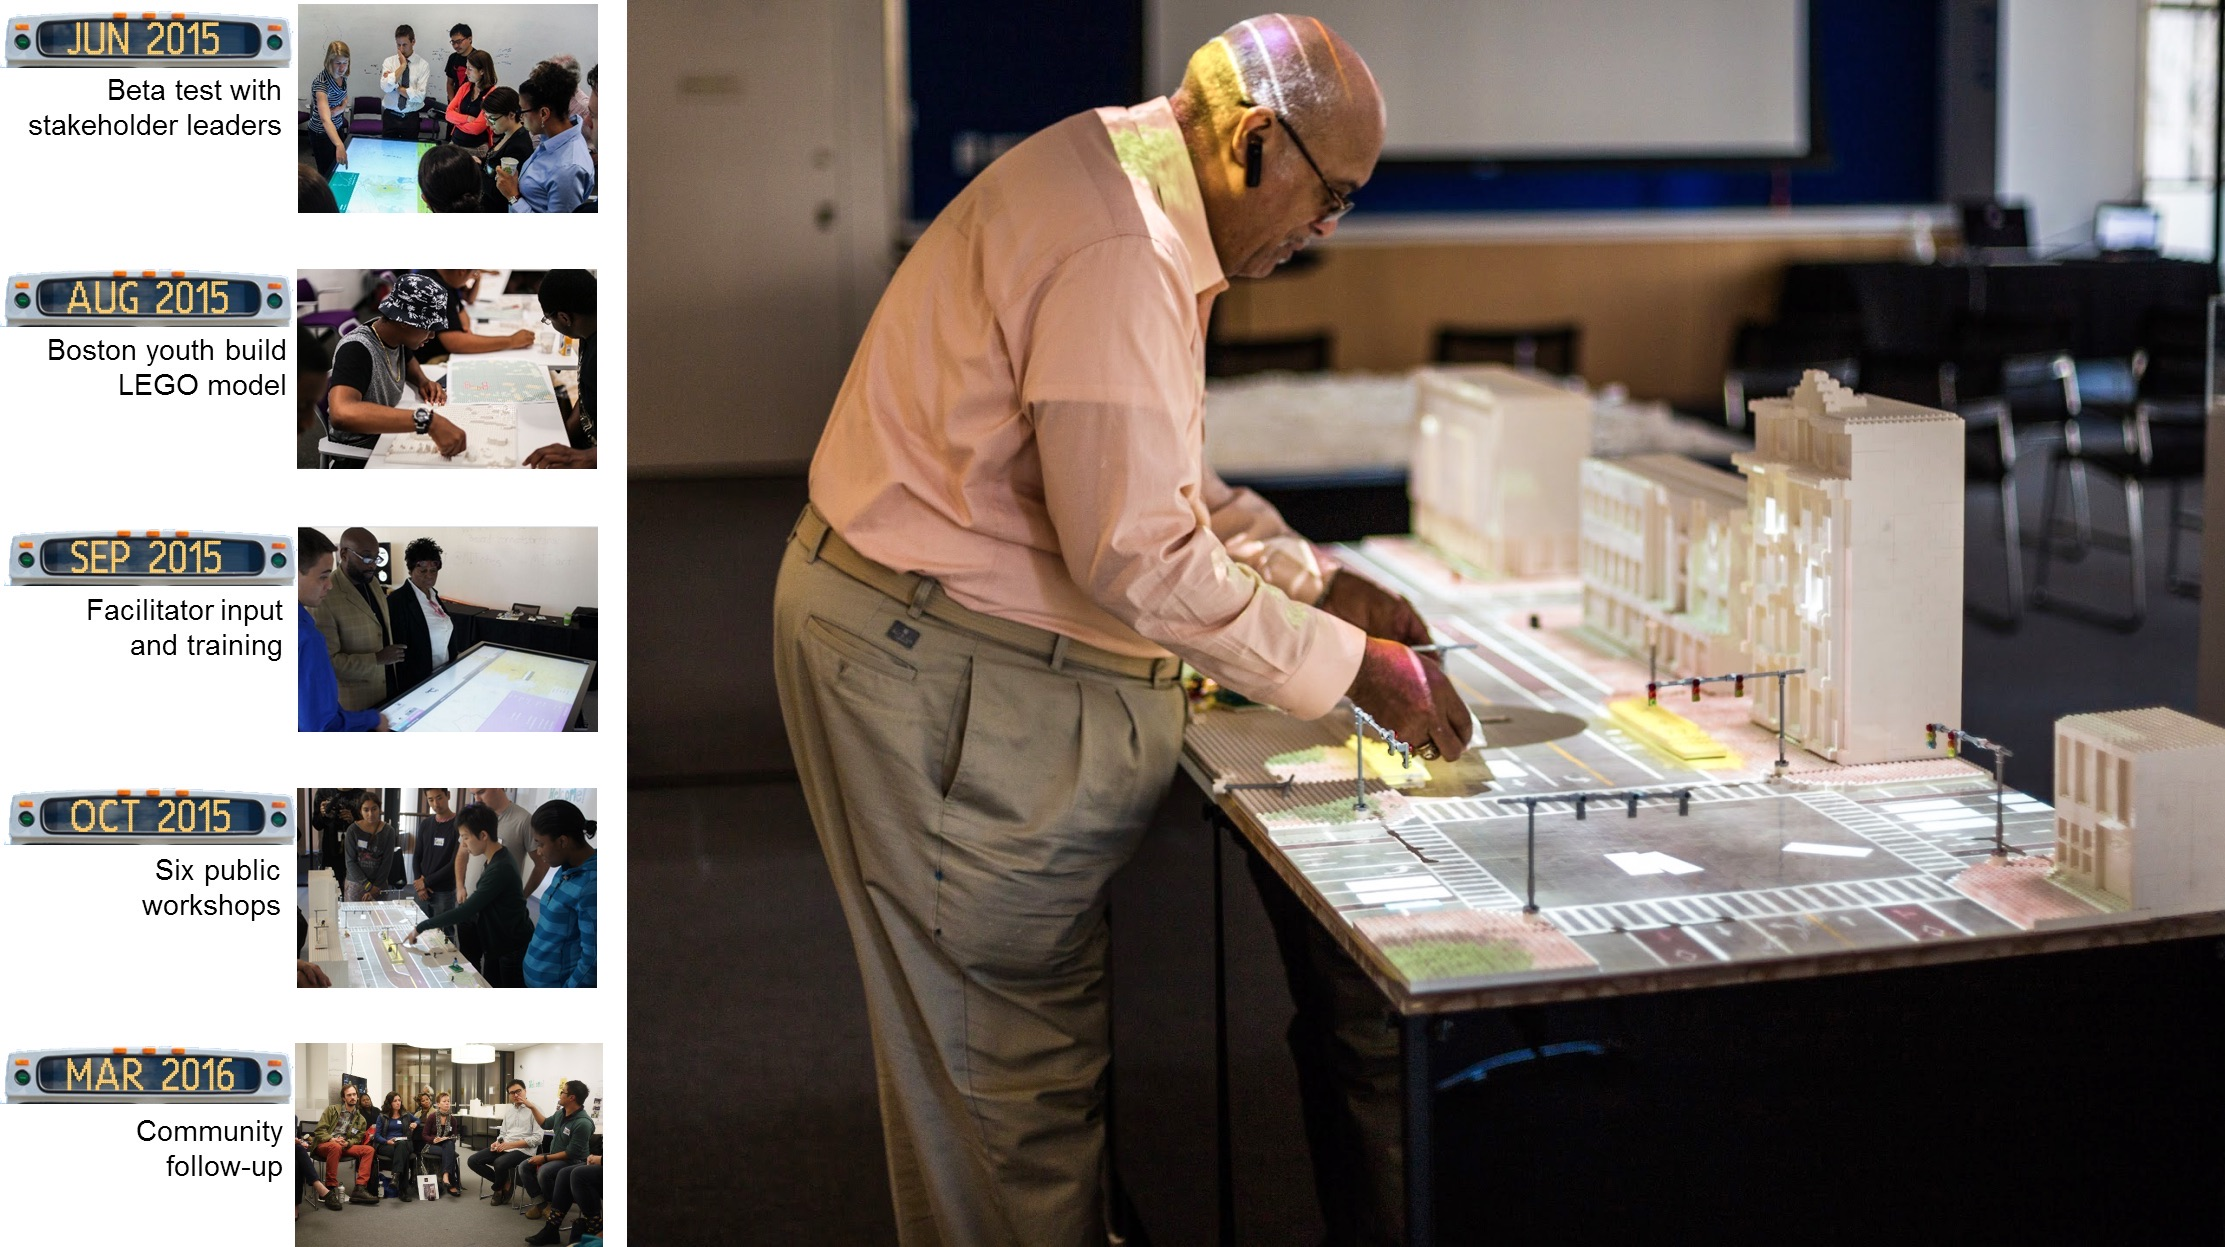
\includegraphics[width=1\textwidth]{chapters/consensus/BRT/figures/brt2.jpeg}
            \end{center}
            \caption{Boston BRT timeline. The community engagement process started months before the actual BRT workshops took place, with activities, co-creation, and constant deliberation with stakeholders and community members. (right) A member of the public operates the BRT Street Scale platform.}
            \label{fig:brt_exit_timeline}
        \end{figure}


        \subsubsection{Research Objectives}
        {
            This project seeks to determine how facilitator-led, collaborative use of new tools might encourage public engagement. Specifically, The research investigates mechanisms to promote social learning, co-creation, and consensus among stakeholders, using collaborative tools in public workshop settings. Potential engagement mechanisms include: (i) Specific features, such as options for localization and interaction based on personal experience; (ii) Tool-supported group interactions, such as discussion and comparison of impacts between user-relevant locations; and (iii) General promotion of understandability, personalization, discussion, teamwork, credibility, and imagination. In testing these mechanisms, participant-reported scores for learning and open dialog are determined from pre-and-post session surveys.
        }


        \begin{figure}[!htb]
            \begin{center}
                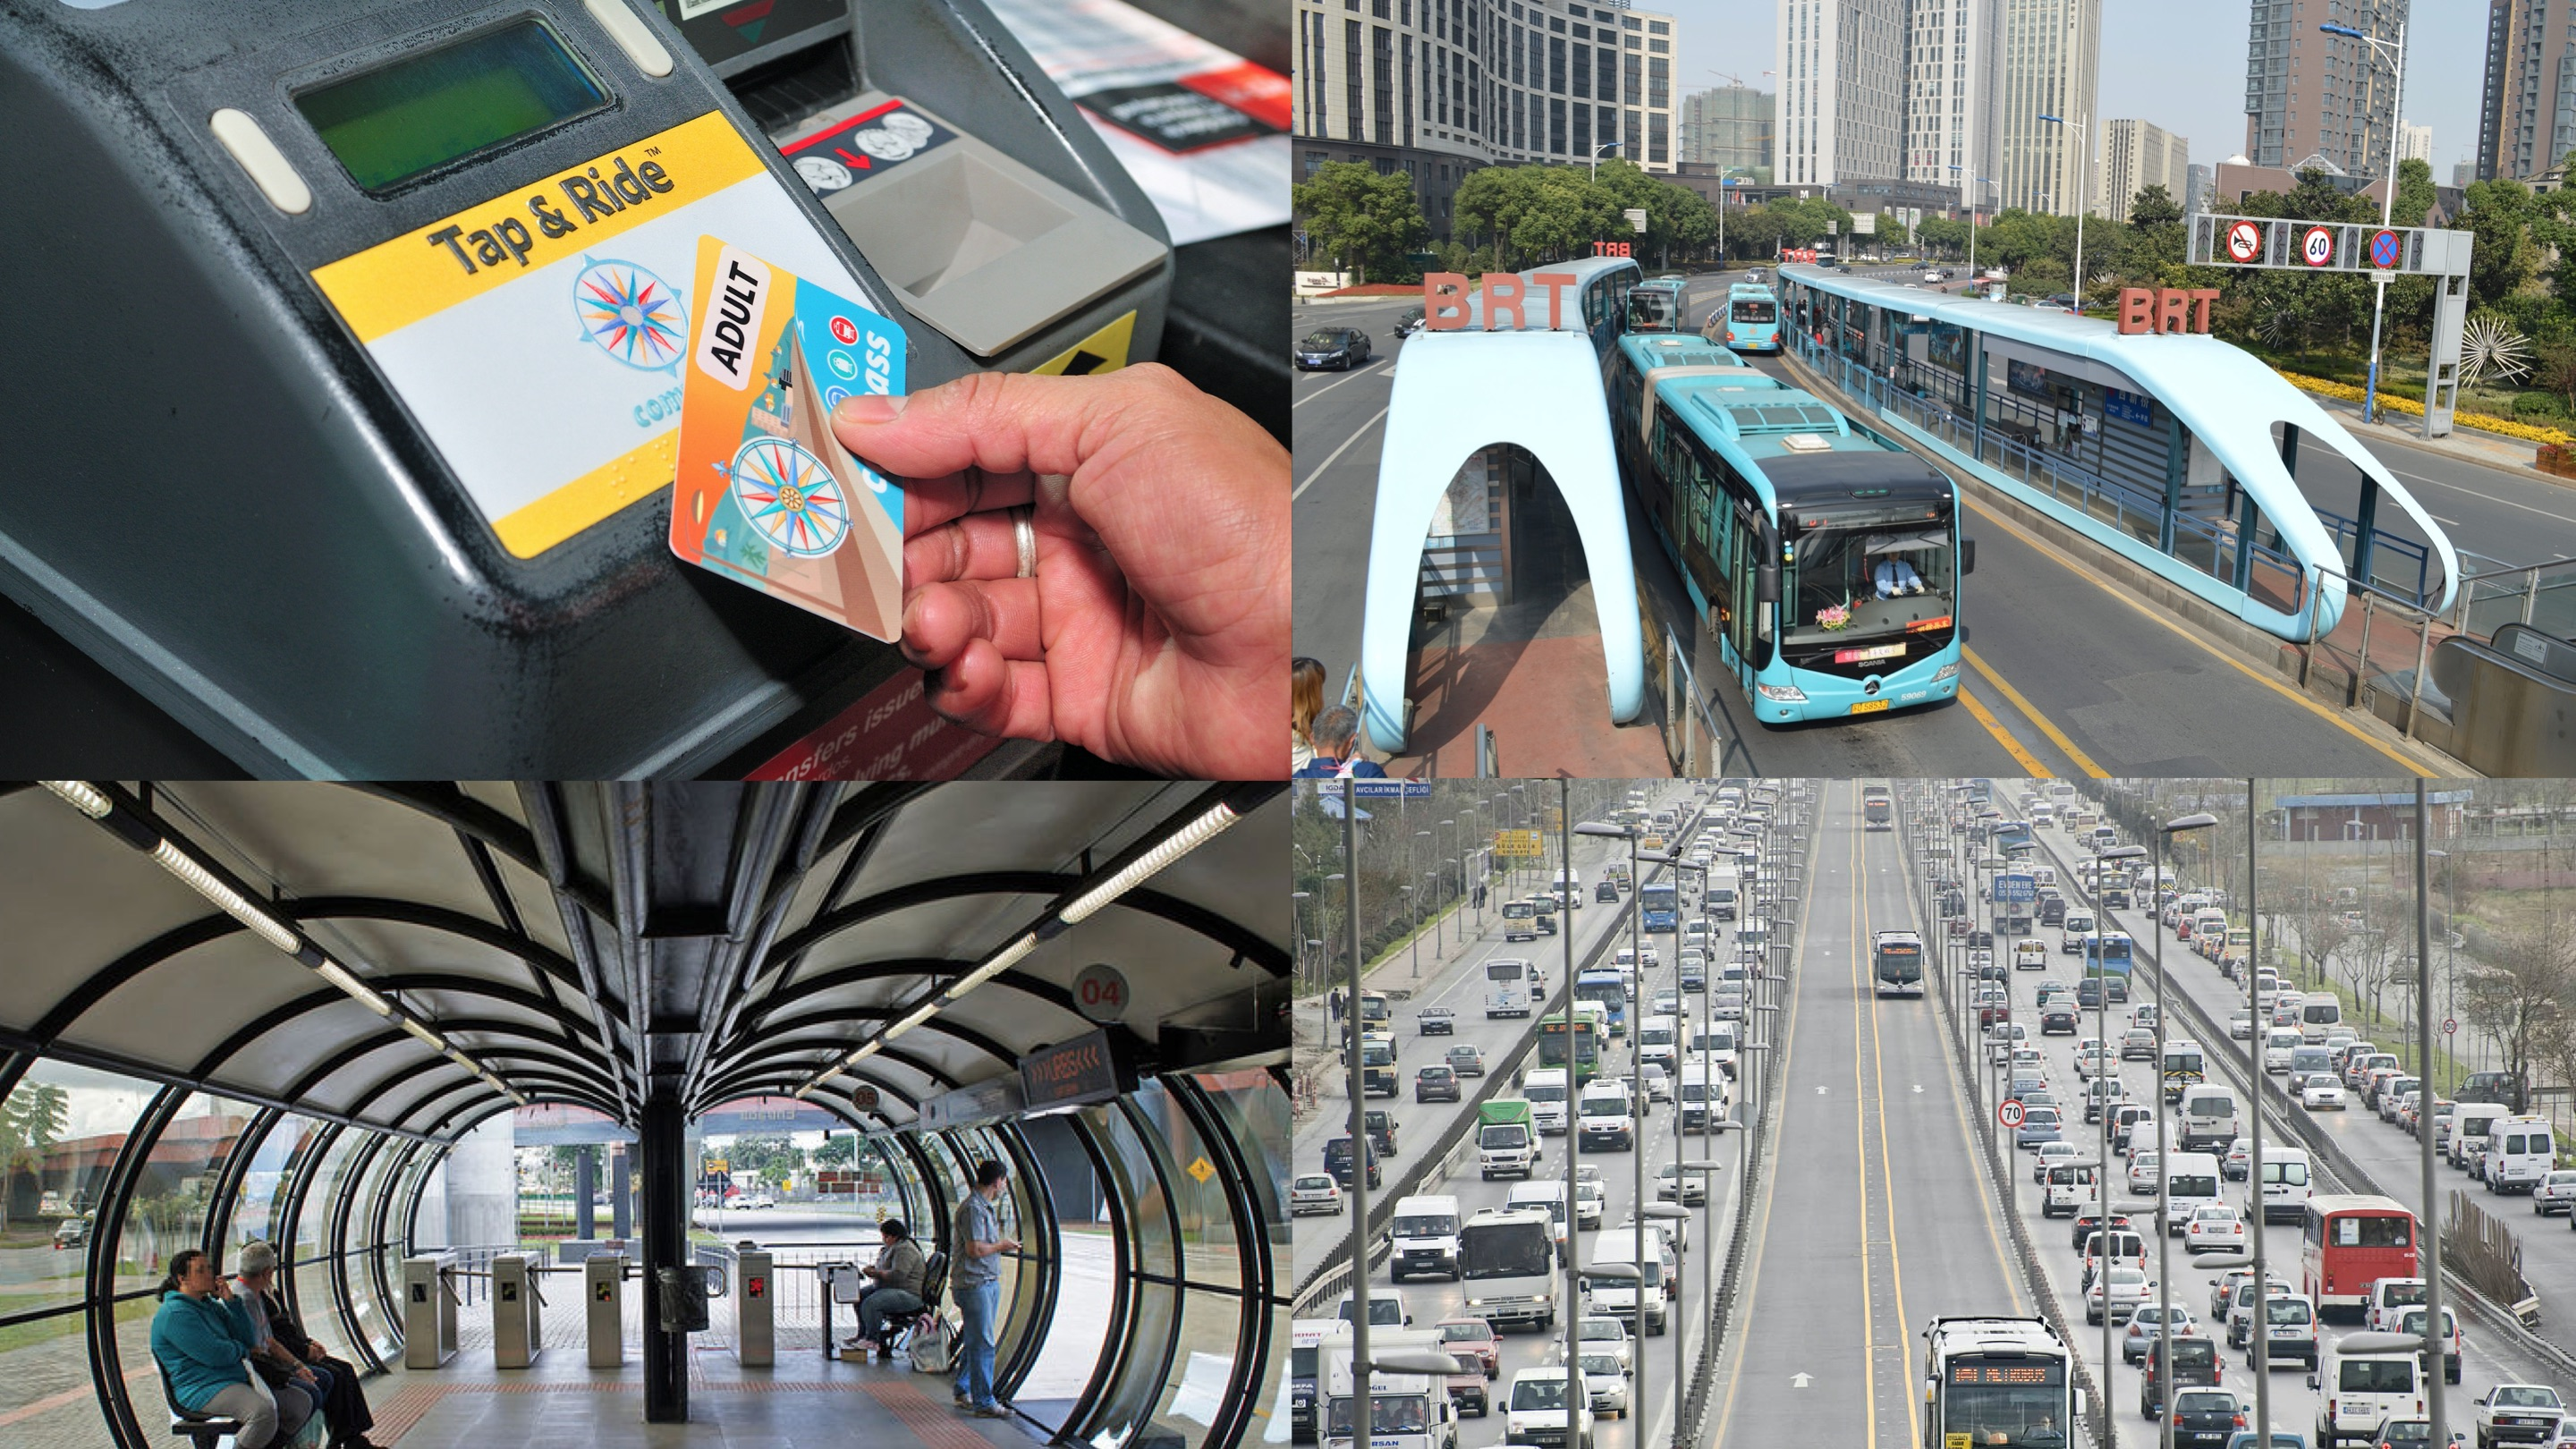
\includegraphics[width=1\textwidth]{chapters/consensus/BRT/figures/brt7.jpeg}
            \end{center}
            \caption{Features of BRT systems \cite{Aboutthe77:online}. At full implementation, a BRT system will feature pre-payment systems, enhanced stations and stops, dedicated lanes, all-door boarding, digital payments, and other features making the BRT experience closer to the performance and convenience of heavy transit solutions.}
            \label{fig:brt_what_is_BRT}
        \end{figure}


        \subsubsection{Bus Rapid Transit}

        {
            Improved bus service can support urban expansion at relatively low cost compared to other mass-transit solutions \cite{williams2015better}. Examples of high quality, bus-based, surface-level public transit exist worldwide, from Mexico City to Malmö (Sweden), and from Cleveland to Cape Town \cite{wirasinghe2013bus}. As Figure \eqref{fig:brt_what_is_BRT} show, these Bus Rapid Transit systems (BRT) tend to include dedicated bus-lanes and pre-payment systems at quality stations. The BRT Standard defines several dozen individual characteristics that the Technical Committee has deemed essential to the definition of BRT. Each is assigned a point value if present; When totaled, the highest scored projects are categorized as `Gold Standard,' followed by `Silver Standard,' and lastly `Bronze Standard.' \cite{Aboutthe77:online}.
            Despite its promise, some aspects of BRT are still controversial: Operating on streets long-dominated by cars can pose difficult tradeoffs in terms of street-scape allocation. BRT might require the removal of existing car lanes or parking spots, change to travel time for car riders, and infrastructural changes to the streetscape \cite{wirasinghe2013bus}.
            \newline
            In 2015, the Greater Boston Bus Rapid Transit Study Group published a report titled \textit{``Better Rapid Transit for Greater Boston: The Potential for Gold Standard Bus Rapid Transit across the Metropolitan Area''} \cite{williams2015better} This document offers a city-wide technical analysis of BRT, and recommends five specific corridors for further evaluation and future implementation. Following the report, The Barr Foundation requested to explore how the use of interactive tools could facilitate the engagement with the community on the wider implications of developing these routes.
        }

        \subsubsection{Site and Context}
        {
            The Roxbury Innovation Center (RIC), Located in the new Bolling Municipal Building in Roxbury (Boston, MA), was selected as the venue location for the community engagement process. RIC sits adjacent to a major bus transportation hub, which is planned to serve several BRT future routes.
            The Roxbury neighborhood has been underserved by transportation and socio-economic mobility for the past several decades \cite{jennings2004urban}. Though Roxbury communities are served by several MBTA bus routes, these operate in mixed traffic and therefore are considerably slower than existing rapid transit lines. Of the fifteen bus routes that are designated by the MBTA as `Key Bus Routes', six provide service in Roxbury, Dorchester, or Mattapan. Five of the MBTA's seven highest ridership bus routes operate primarily within these neighborhoods \cite{MapsMBTA95:online}. These routes tend to suffer from poor reliability, slow travel speeds, overcrowding, and a lack of customer amenities \cite{SurveyBo15:online}. Of the five potential corridors proposed in the BRT Study Group report, three converge at the Dudley Square station, making Roxbury an ideal community for stakeholders engagement in the evaluation of BRT potential \cite{williams2015better}.
        }
    }

    \begin{figure}[!htb]
        \begin{center}
            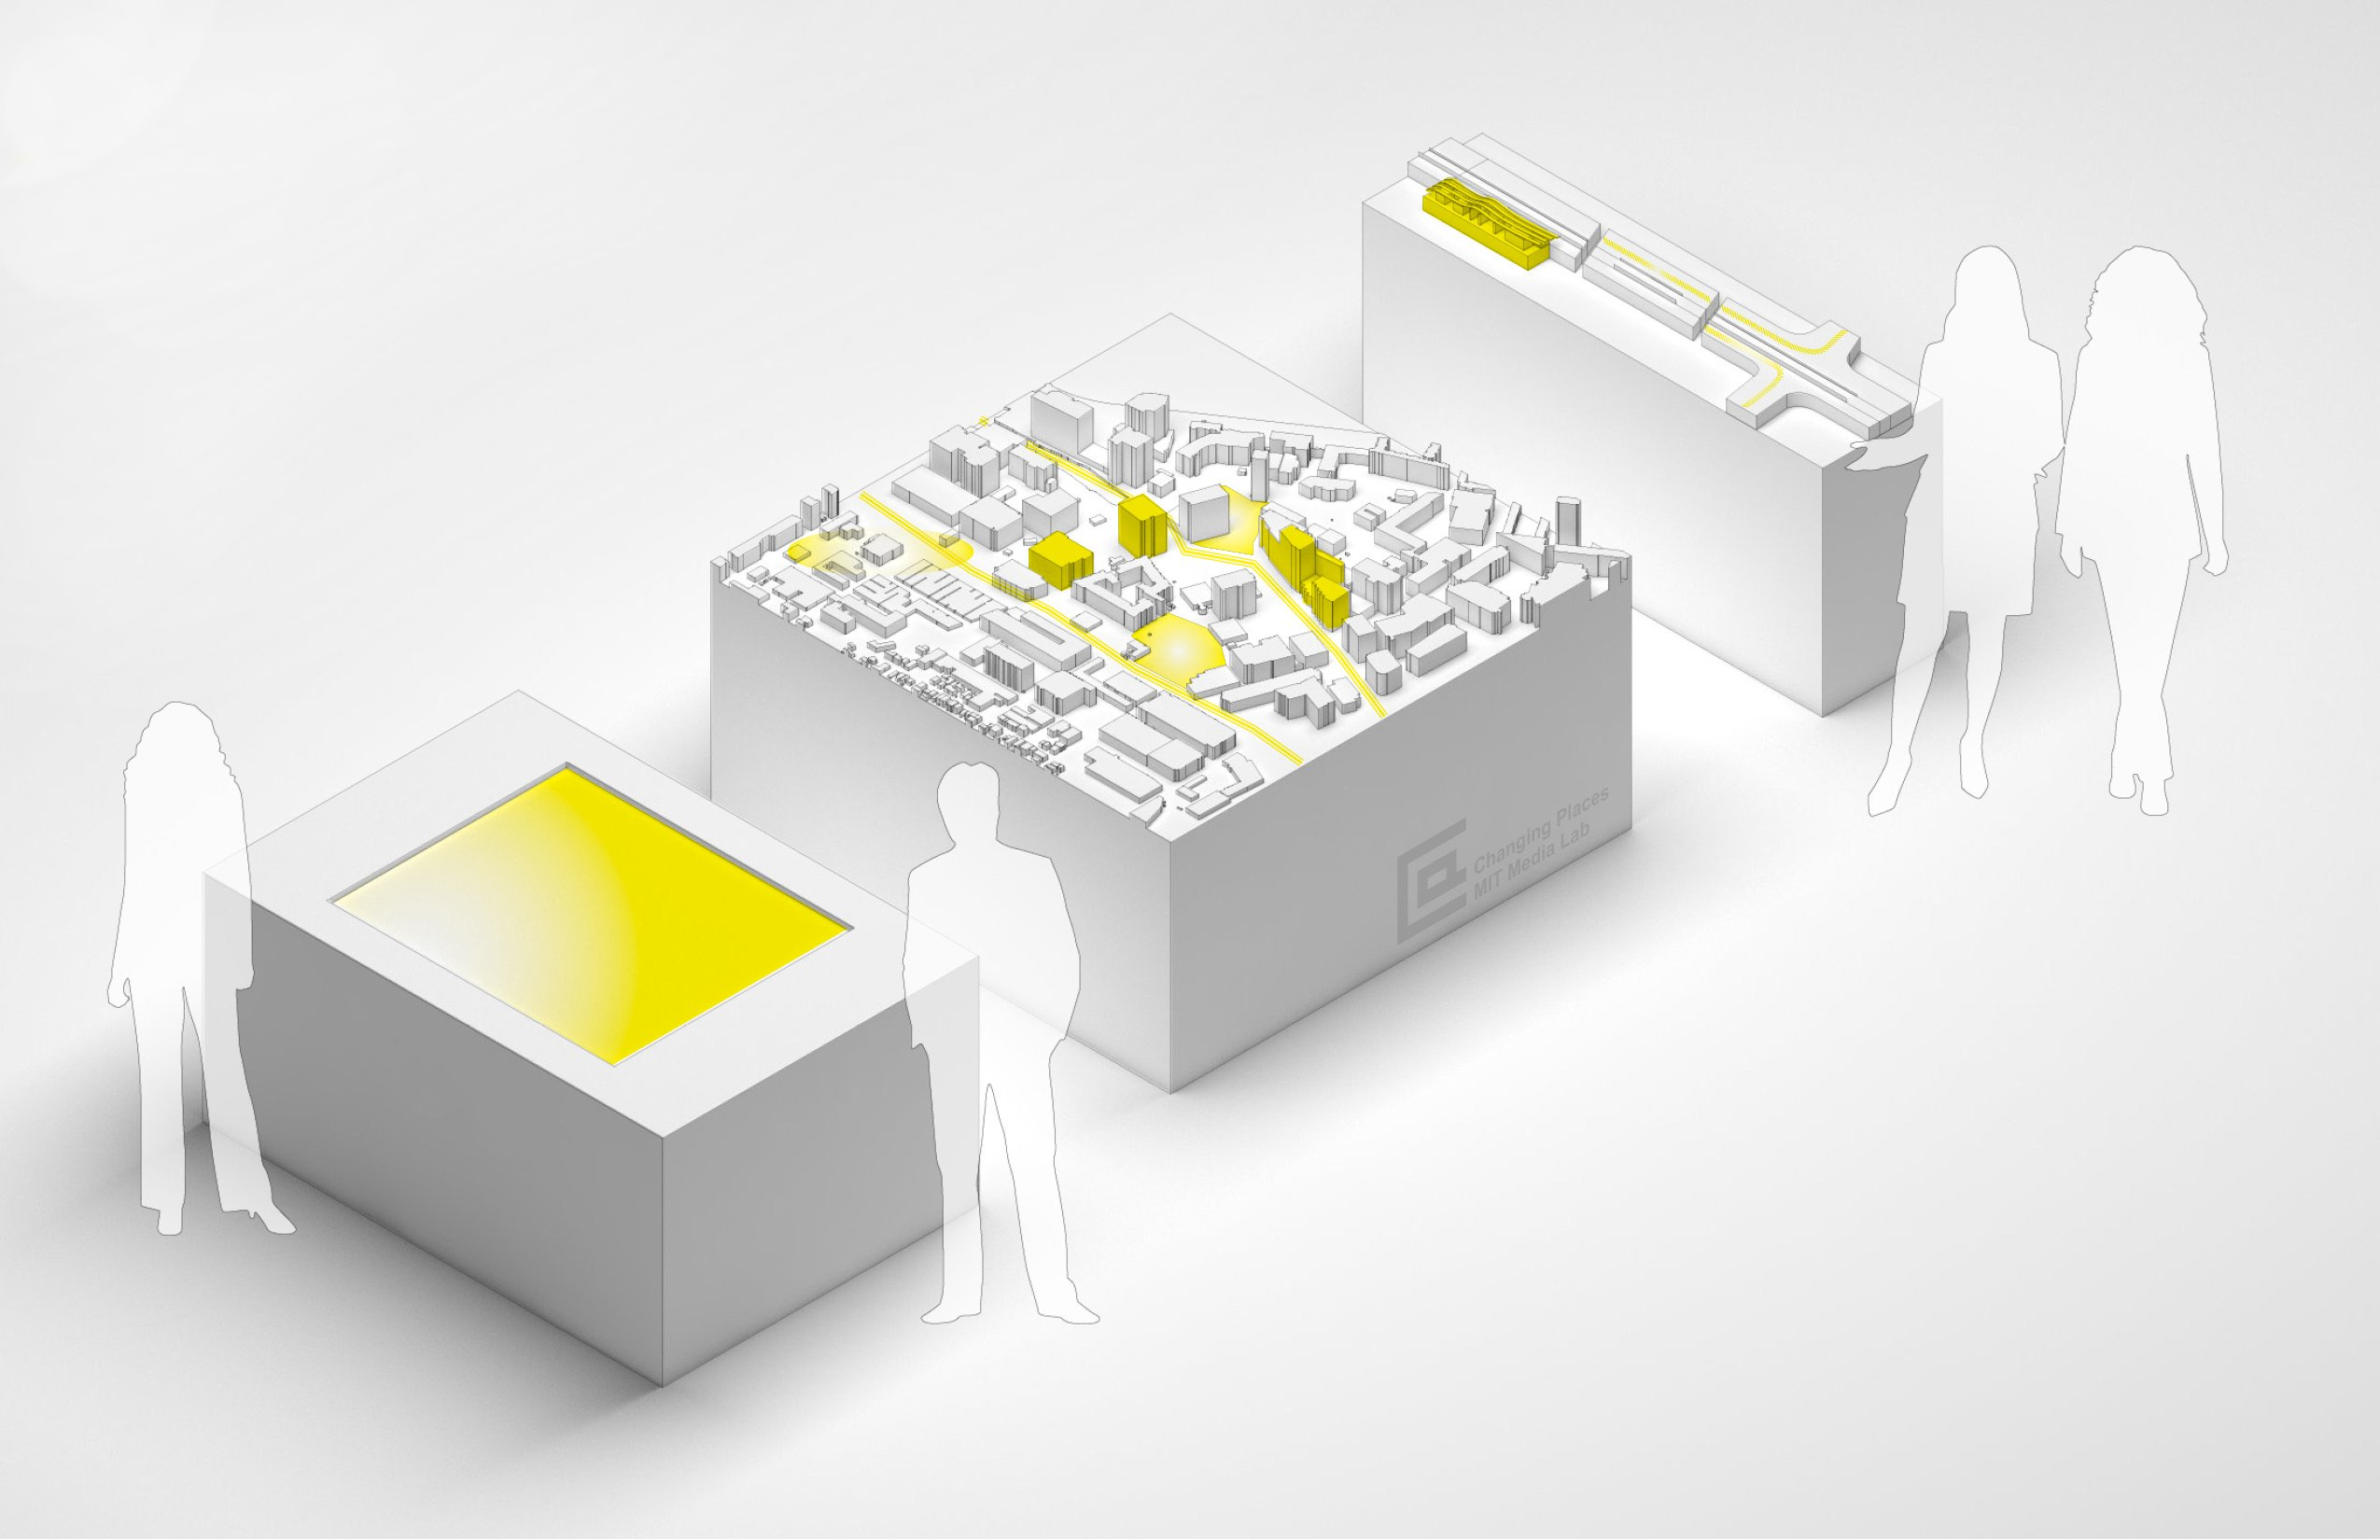
\includegraphics[width=1\textwidth]{chapters/consensus/BRT/figures/brt0.jpeg}
        \end{center}
        \caption{CityScope BRT. Three CityScope instances were proposed to allow simultaneous discussions in multiple scales and different impact levels of the BRT system. The three platforms also presented a gradual move from an intuitive street-scale tool to a more detailed and complex regional platform.}
        \label{fig:brt_platforms}
    \end{figure}

    \subsection{CityScope Tools}
    {
        A set of tools was developed in an effort to test collaboration and co-creation using digital platforms in the context of BRT planning. These include CoAXs \cite{stewart2016coaxs}, a web-based interactive platform for collaborative transit planning\footnote{CoAXs was built upon the open-source urban analytics tool Conveyal \cite{Conveyal33:online}. For a detailed description of CoAXs, see \cite{stewart2016coaxs}}. The second set of tools were two CityScope platforms, designed for the neighborhood and street-level scales. These offered an iterative way to examine alternatives for bus corridor designs, station types, street layouts, as well as travel times and environmental impacts. CityScope visualized traffic based on the outputs of different analysis tools such as SUMO, an open source traffic modeling software \cite{krajzewicz2012recent}. The following section details the tools and their functionality.

        \begin{figure}[!htb]
            \begin{center}
                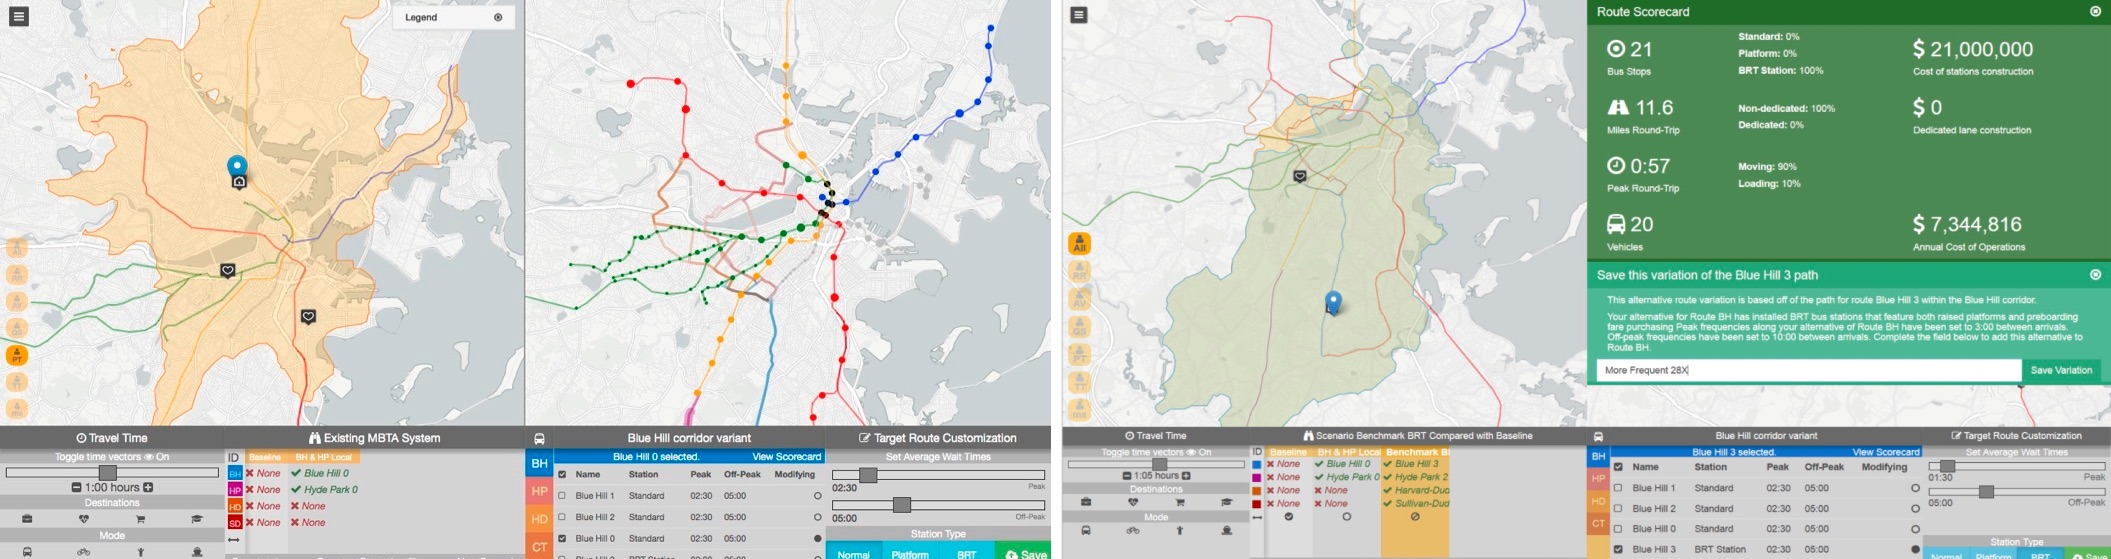
\includegraphics[width=1\textwidth]{chapters/consensus/BRT/figures/brt4.jpeg}
            \end{center}
            \caption{CoAXs regional scale UI. These screen-captures show the control panel and interaction with the CoAXs touch screen interface, with results from the Conveyal accessibility service, including assessed travel time, access to different amenities and functions, as well as estimated cost.}
            \label{fig:brt_street_CoAXs}
        \end{figure}

        \subsubsection{CoAXs: Regional Scale}
        {
            CoAXs (short for `Co-Creative Accessibility-Based Stakeholder Engagement') is a web-based mapping and visualization tool designed to evaluate and communicate benefits of transit projects in collaborative planning. CoAXs seeks to link maps and accessibility indices with various common travel patterns. For example, viewers can point to a specific location in the city (via interactive touch interface) and learn their access to job locations given proposed public transportation. They can then control various model assumptions (such as bus frequency) to see how different transit systems and route networks affect their commute as well as overall job accessibility.
            \newline
            CoAXs has two modules: (i) the accessibility analyst, synthesize data about transit service, pedestrian and cycling networks, land-use, and socio-economics, to provide interactive maps of both individual access to opportunities and regional accessibility; (ii) a sketch-planning corridor editor that allows users to modify the service parameters of bus corridors and create different corridors` scenarios.
            CoAX is built using Conveyal's Transport Analyst and Open Trip Planner \cite{Conveyal33:online}.
        }


        \begin{figure}[!htb]
            \begin{center}
                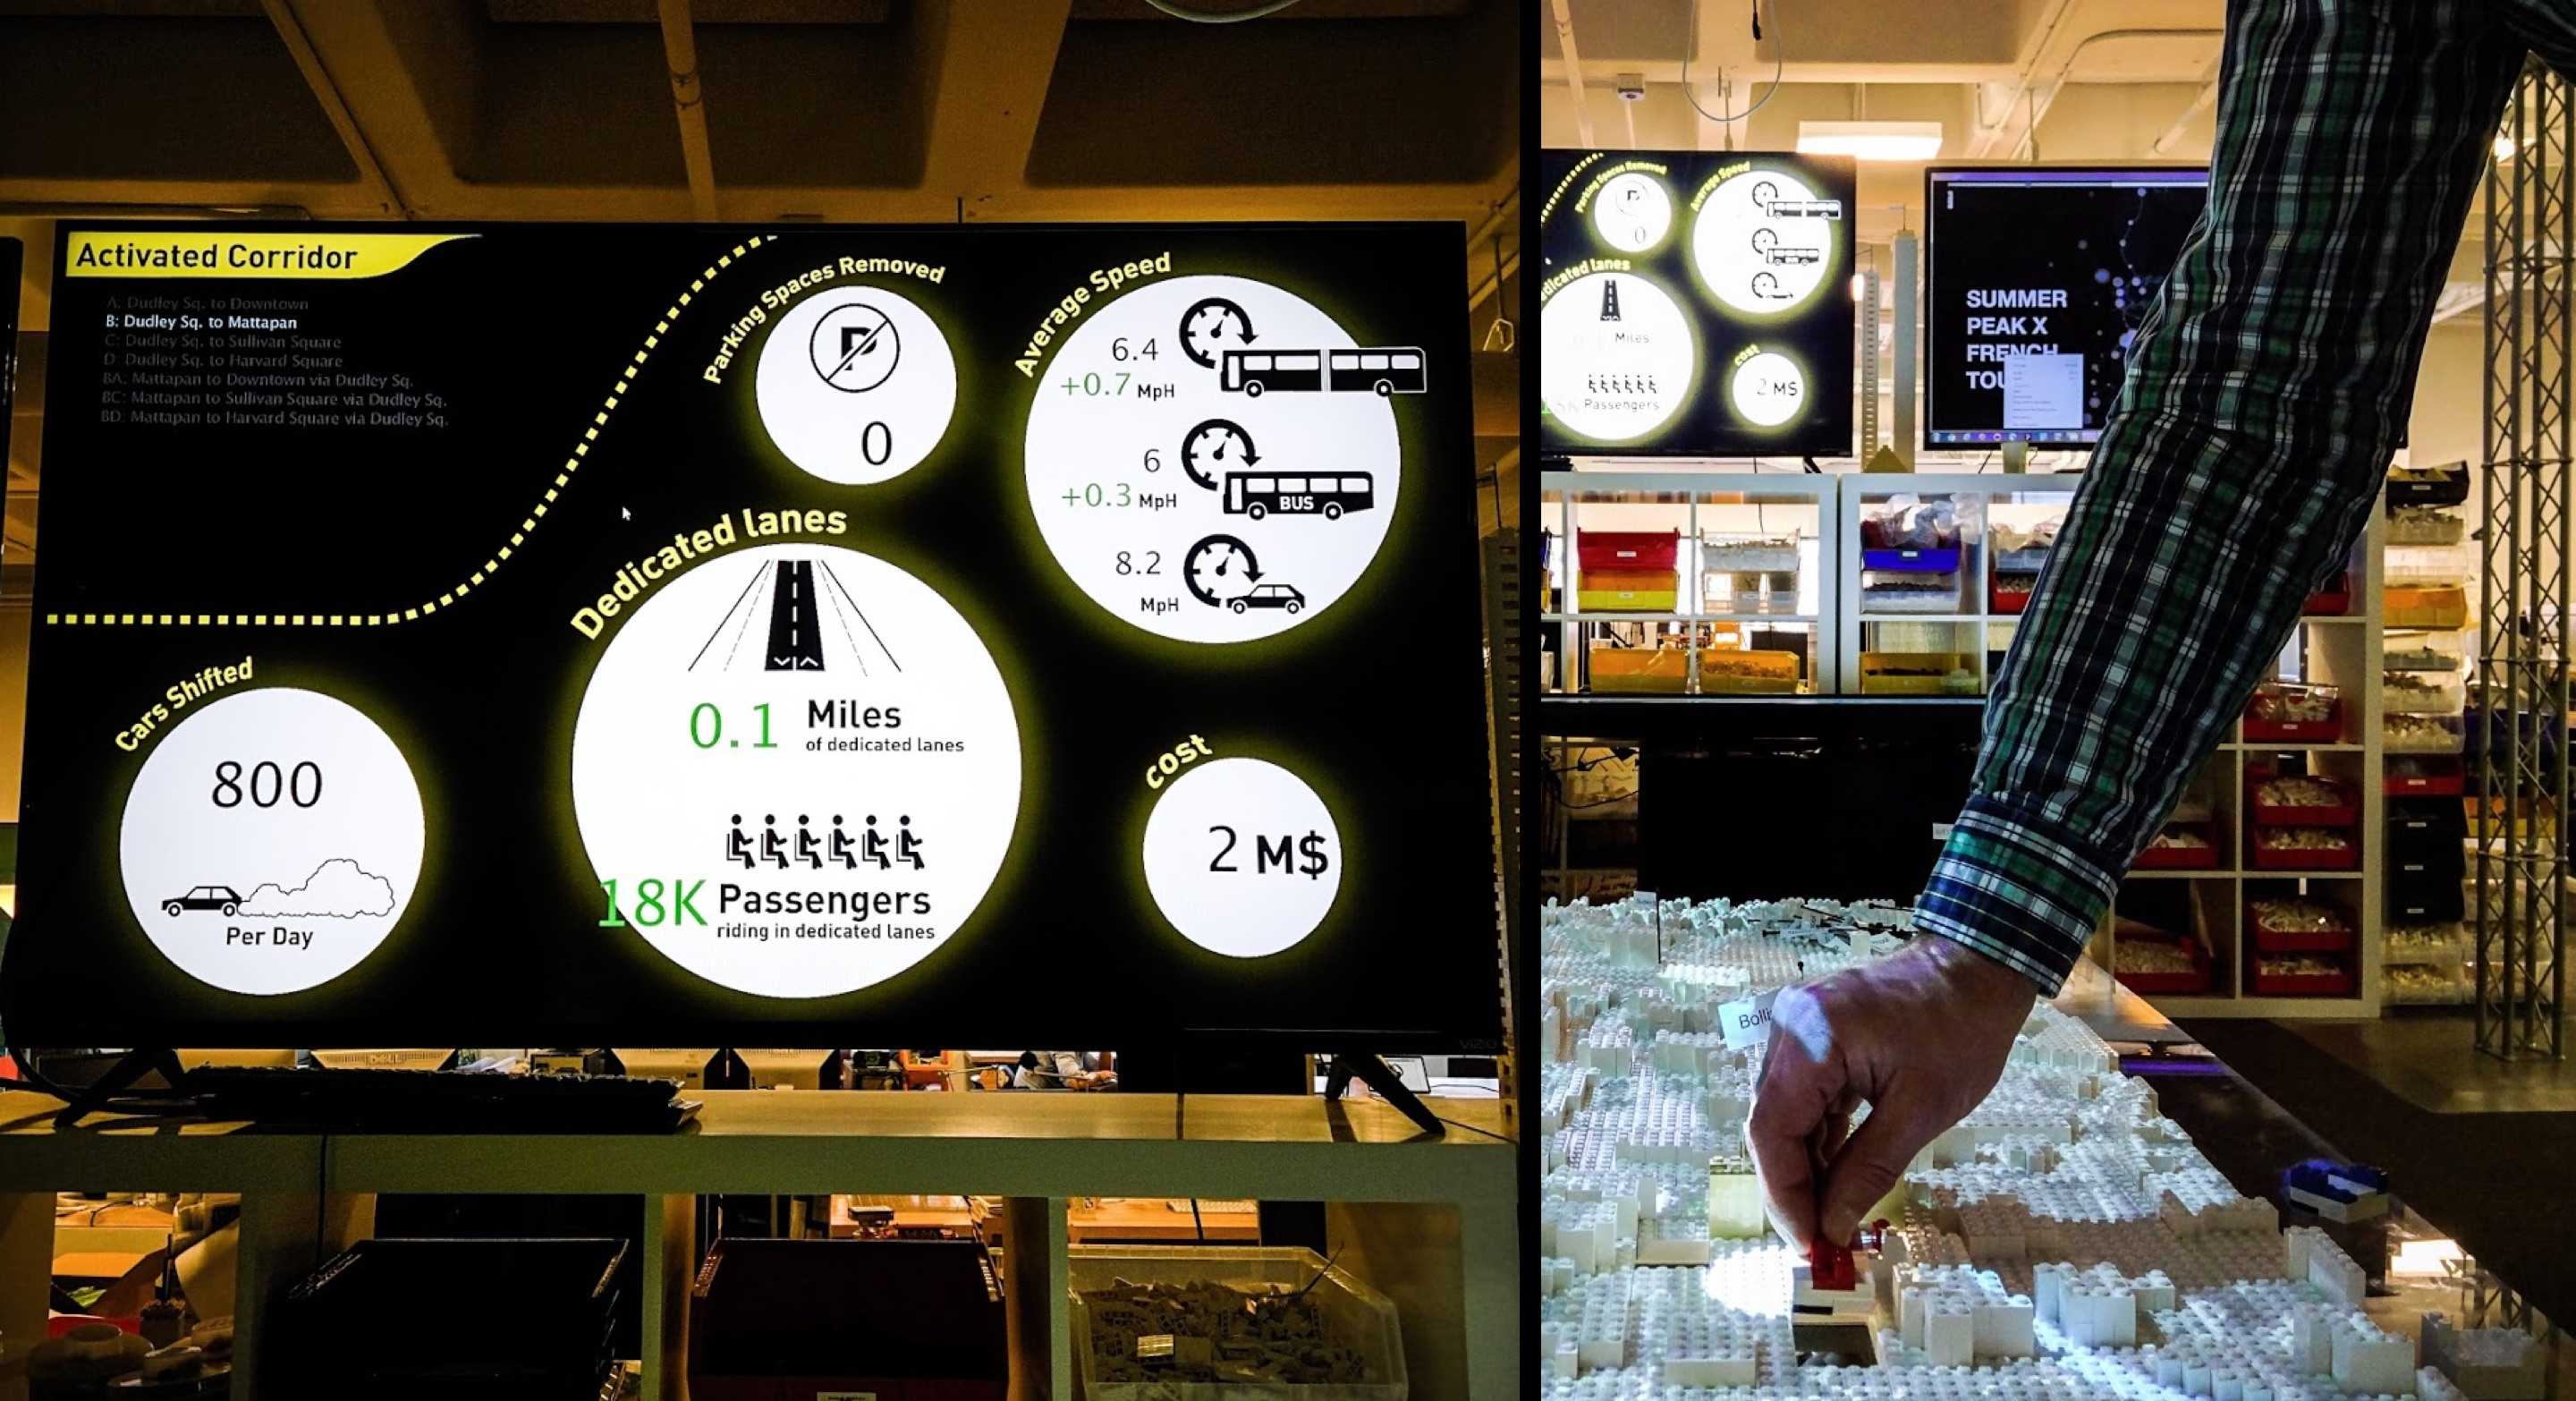
\includegraphics[width=.8\textwidth]{chapters/consensus/BRT/figures/brt11.jpeg}
            \end{center}
            \caption{Neighborhood Scale. This TUI responded to users' changing the BRT tiers with highlighted routes, travel times, cost, and environmental impacts. Between the three platforms, the Neighborhood scale was the least useful, as the tangible interface did not contribute to the understanding of the BRT system, and the coarseness of the model was found to be confusing.}
            \label{fig:brt_neighborhood_scale}
        \end{figure}


        \subsubsection{CityScope: Neighborhood and Street Scales}
        {
            Two CityScope instances were designed for the analysis of BRT systems, neighborhood and street Scales. These complement the CoAXs modules, and allow users to explore the potential impacts of different BRT configurations and route networks of neighborhoods and streets.


            \begin{figure}[!htb]
                \begin{center}
                    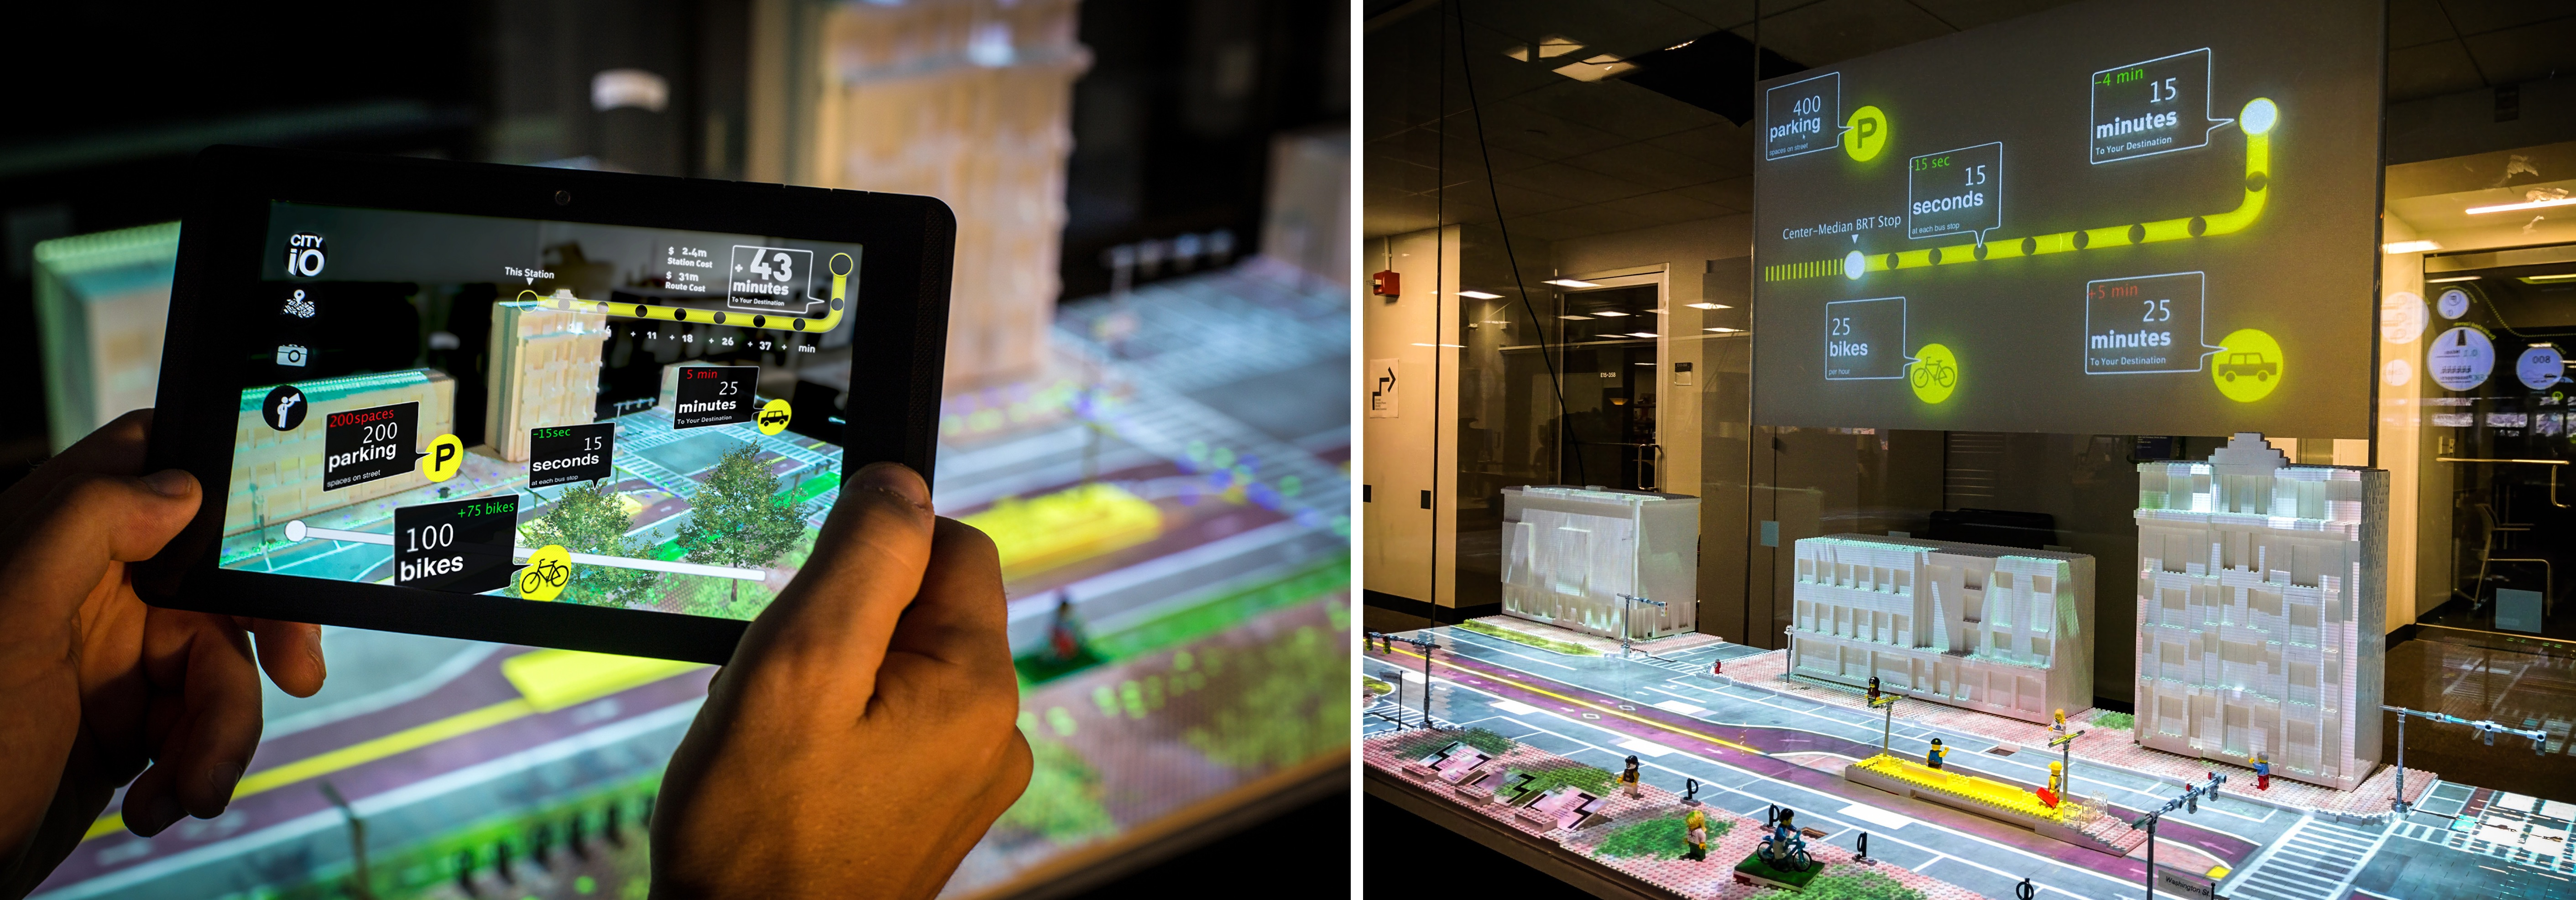
\includegraphics[width=1\textwidth]{chapters/consensus/BRT/figures/brt6.jpeg}
                \end{center}
                \caption{BRT `Street-Scale'. As users interact with the TUI (right), both the projection and AR device (left) update information about the impacts of the different BRT tiers.}
                \label{fig:brt_street}
            \end{figure}

            \textbf{Neighborhood:} The Neighborhood scale is designed to explore the accessibility created using new BRT routes in the vicinity of the Roxbury area. This scale provides users with a design-decisions interface around selection of street corridors, placement and sizing of stations, and improving overall utilization of transit systems. A 3D neighborhood scale model was fitted with several placements for inserting LEGO tiles, which refer to BRT stations in key locations across the city. Each of the bricks would represent one of three BRT station standards (Gold, Silver, or Bronze. See \cite{Aboutthe77:online}). When users place a station onto the designated spot, the corresponding BRT route and its stations are displayed. In addition, recorded BRT trips simulation is playing, showing a fast-paced visualization of the proposed routes for this BRT class. The selected type of the BRT class also impacts several precalculated metrics, such as the number of passengers served, the number of trips per hour, as well as environmental impacts. These are displayed on auxiliary monitors.

            \begin{figure}[!htb]
                \begin{center}
                    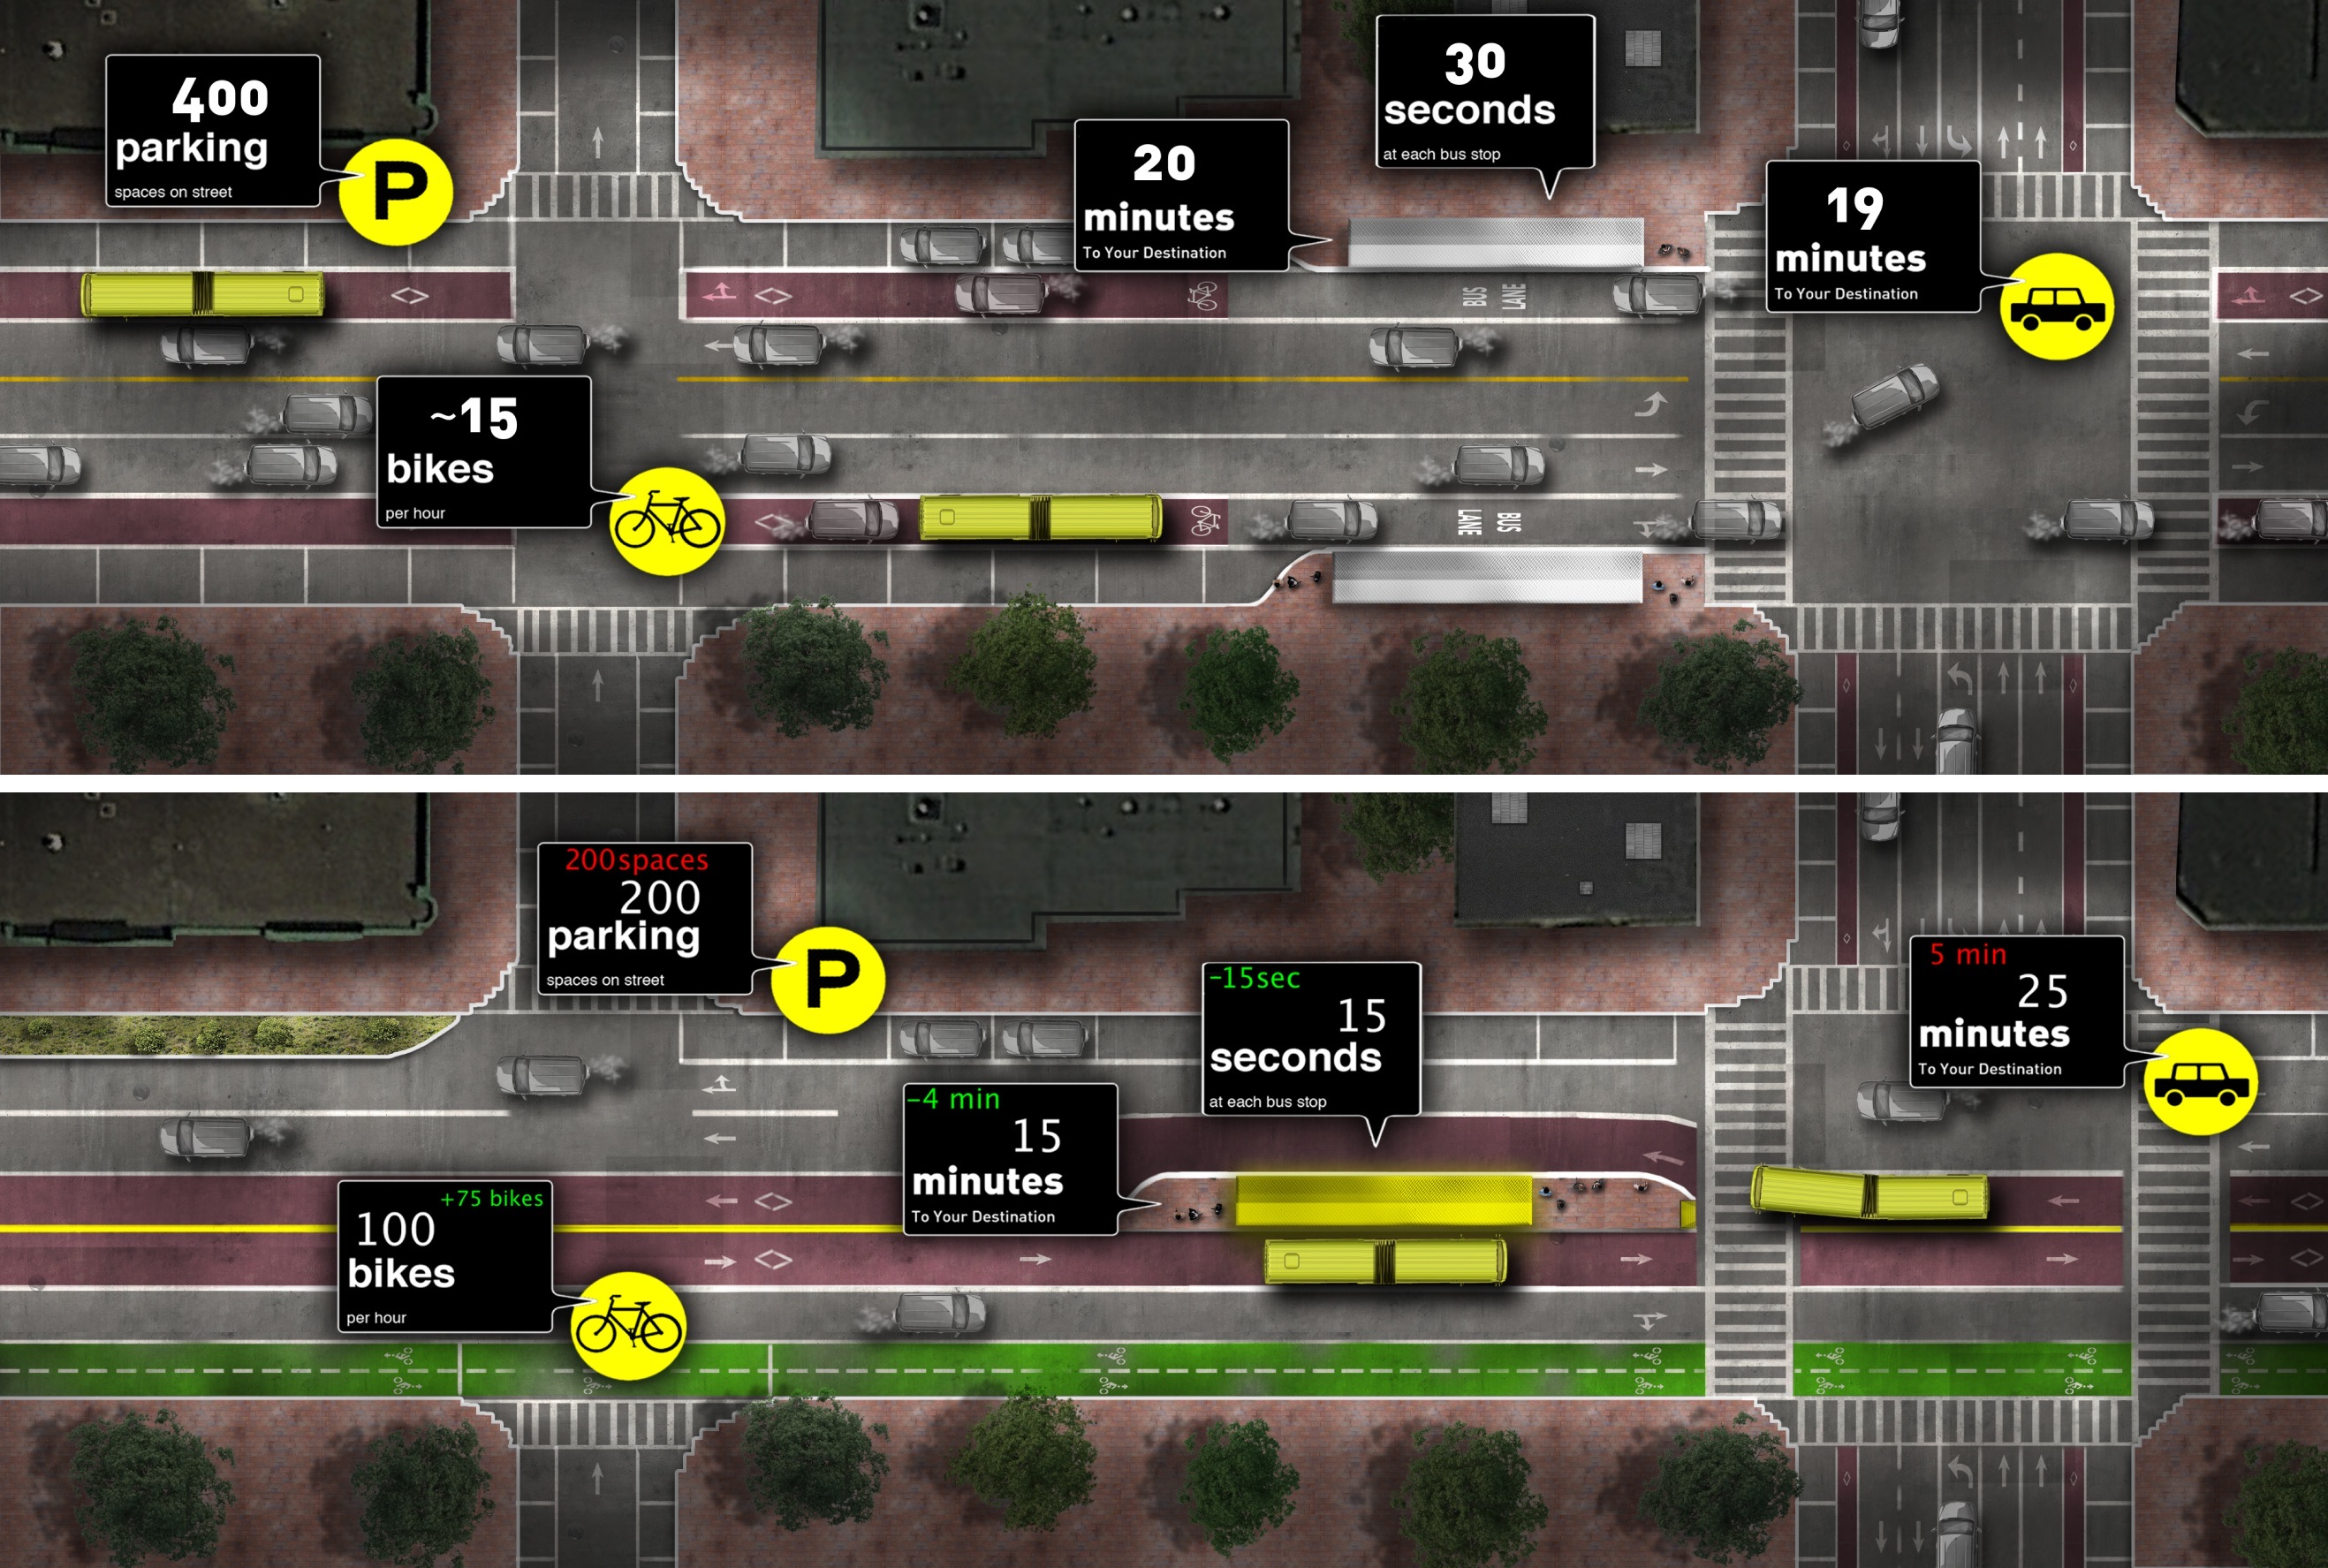
\includegraphics[width=1\textwidth]{chapters/consensus/BRT/figures/brt3.jpeg}
                \end{center}
                \caption{Street-Scale TUI screen-captures. (top) Washington st. in its current state, including the performance of the MBTA Silver Line, available parking, and bike access. (bottom) Washington st. fitted with a `BRT Gold Standard', including improved transit times and accuracy, enhanced bike access, and tradeoffs to private vehicles.}
                \label{fig:brt_street_viz}
            \end{figure}

            \textbf{Street:} The second instance focuses on the street-level impacts of a BRT corridor. This street section was modelled after a segment of Washington st., which included an existing MBTA Silver Line bus route. Here, users are promoted to engage in design-decisions such as placement and sizing of various stations, streetscape design, bike-able access to BRT stations, and increasing access for seniors, disabled, and youth. Users can switch out different pieces representing various types of bus stops (from traditional ones to high-tech stations where riders pay before they board) and observe the simulated change in traffic flow on the LEGO platform. Data about the bus station's efficiency is also projected on nearby screens, as well as on the CityScopeAR platform \cite{nsl19}.
        }
    }

    \subsection{Workshops}
    {
        The development of the different tools took place during the first half of 2015. As part of the engagement process, Boston high school students participating in the MLK Scholars program, constructed the neighborhood scale LEGO model of Roxbury. Between June and October, several review sessions and workshops were held at the MIT Media Lab, hosting stakeholders, members of the community, and students participants. In September, the three tools were deployed to the venue site, and facilitators training session took place at MIT and on the venue premise. During October, six workshops, involving 53 participation, took place in the venue. Alongside the workshops, the venue was open for members of the community to explore the CityScope tools and learn about the proposed BRT system. The following section details the workshops, agenda, and feedback collection.

        \subsubsection{Facilitators}
        {
            Typically problematic of government-run community meetings is the perception that control of the technology, and therefore the analyses, is in the hands of technical experts \cite{innes2010planning, arnstein1969ladder}. By combining interactive tools with community facilitators, participants' perception of tools credibility and empowerment to play a more active role in planning their own community was tested.
            \newline
            A key element of the workshops was the partnership with Nuestra Communidad \cite{nuestracdc:online} who provided six members as facilitators for the workshops. Rather than have researchers engaging the public, community leaders facilitated the workshops sessions and operated the tools by themselves. Two training sessions were held with the facilitators prior to the workshops; An unintended benefit of these training sessions was the valuable feedback on the tools' usability, readability, and accessibility.
        }

        \begin{figure}[!htb]
            \begin{center}
                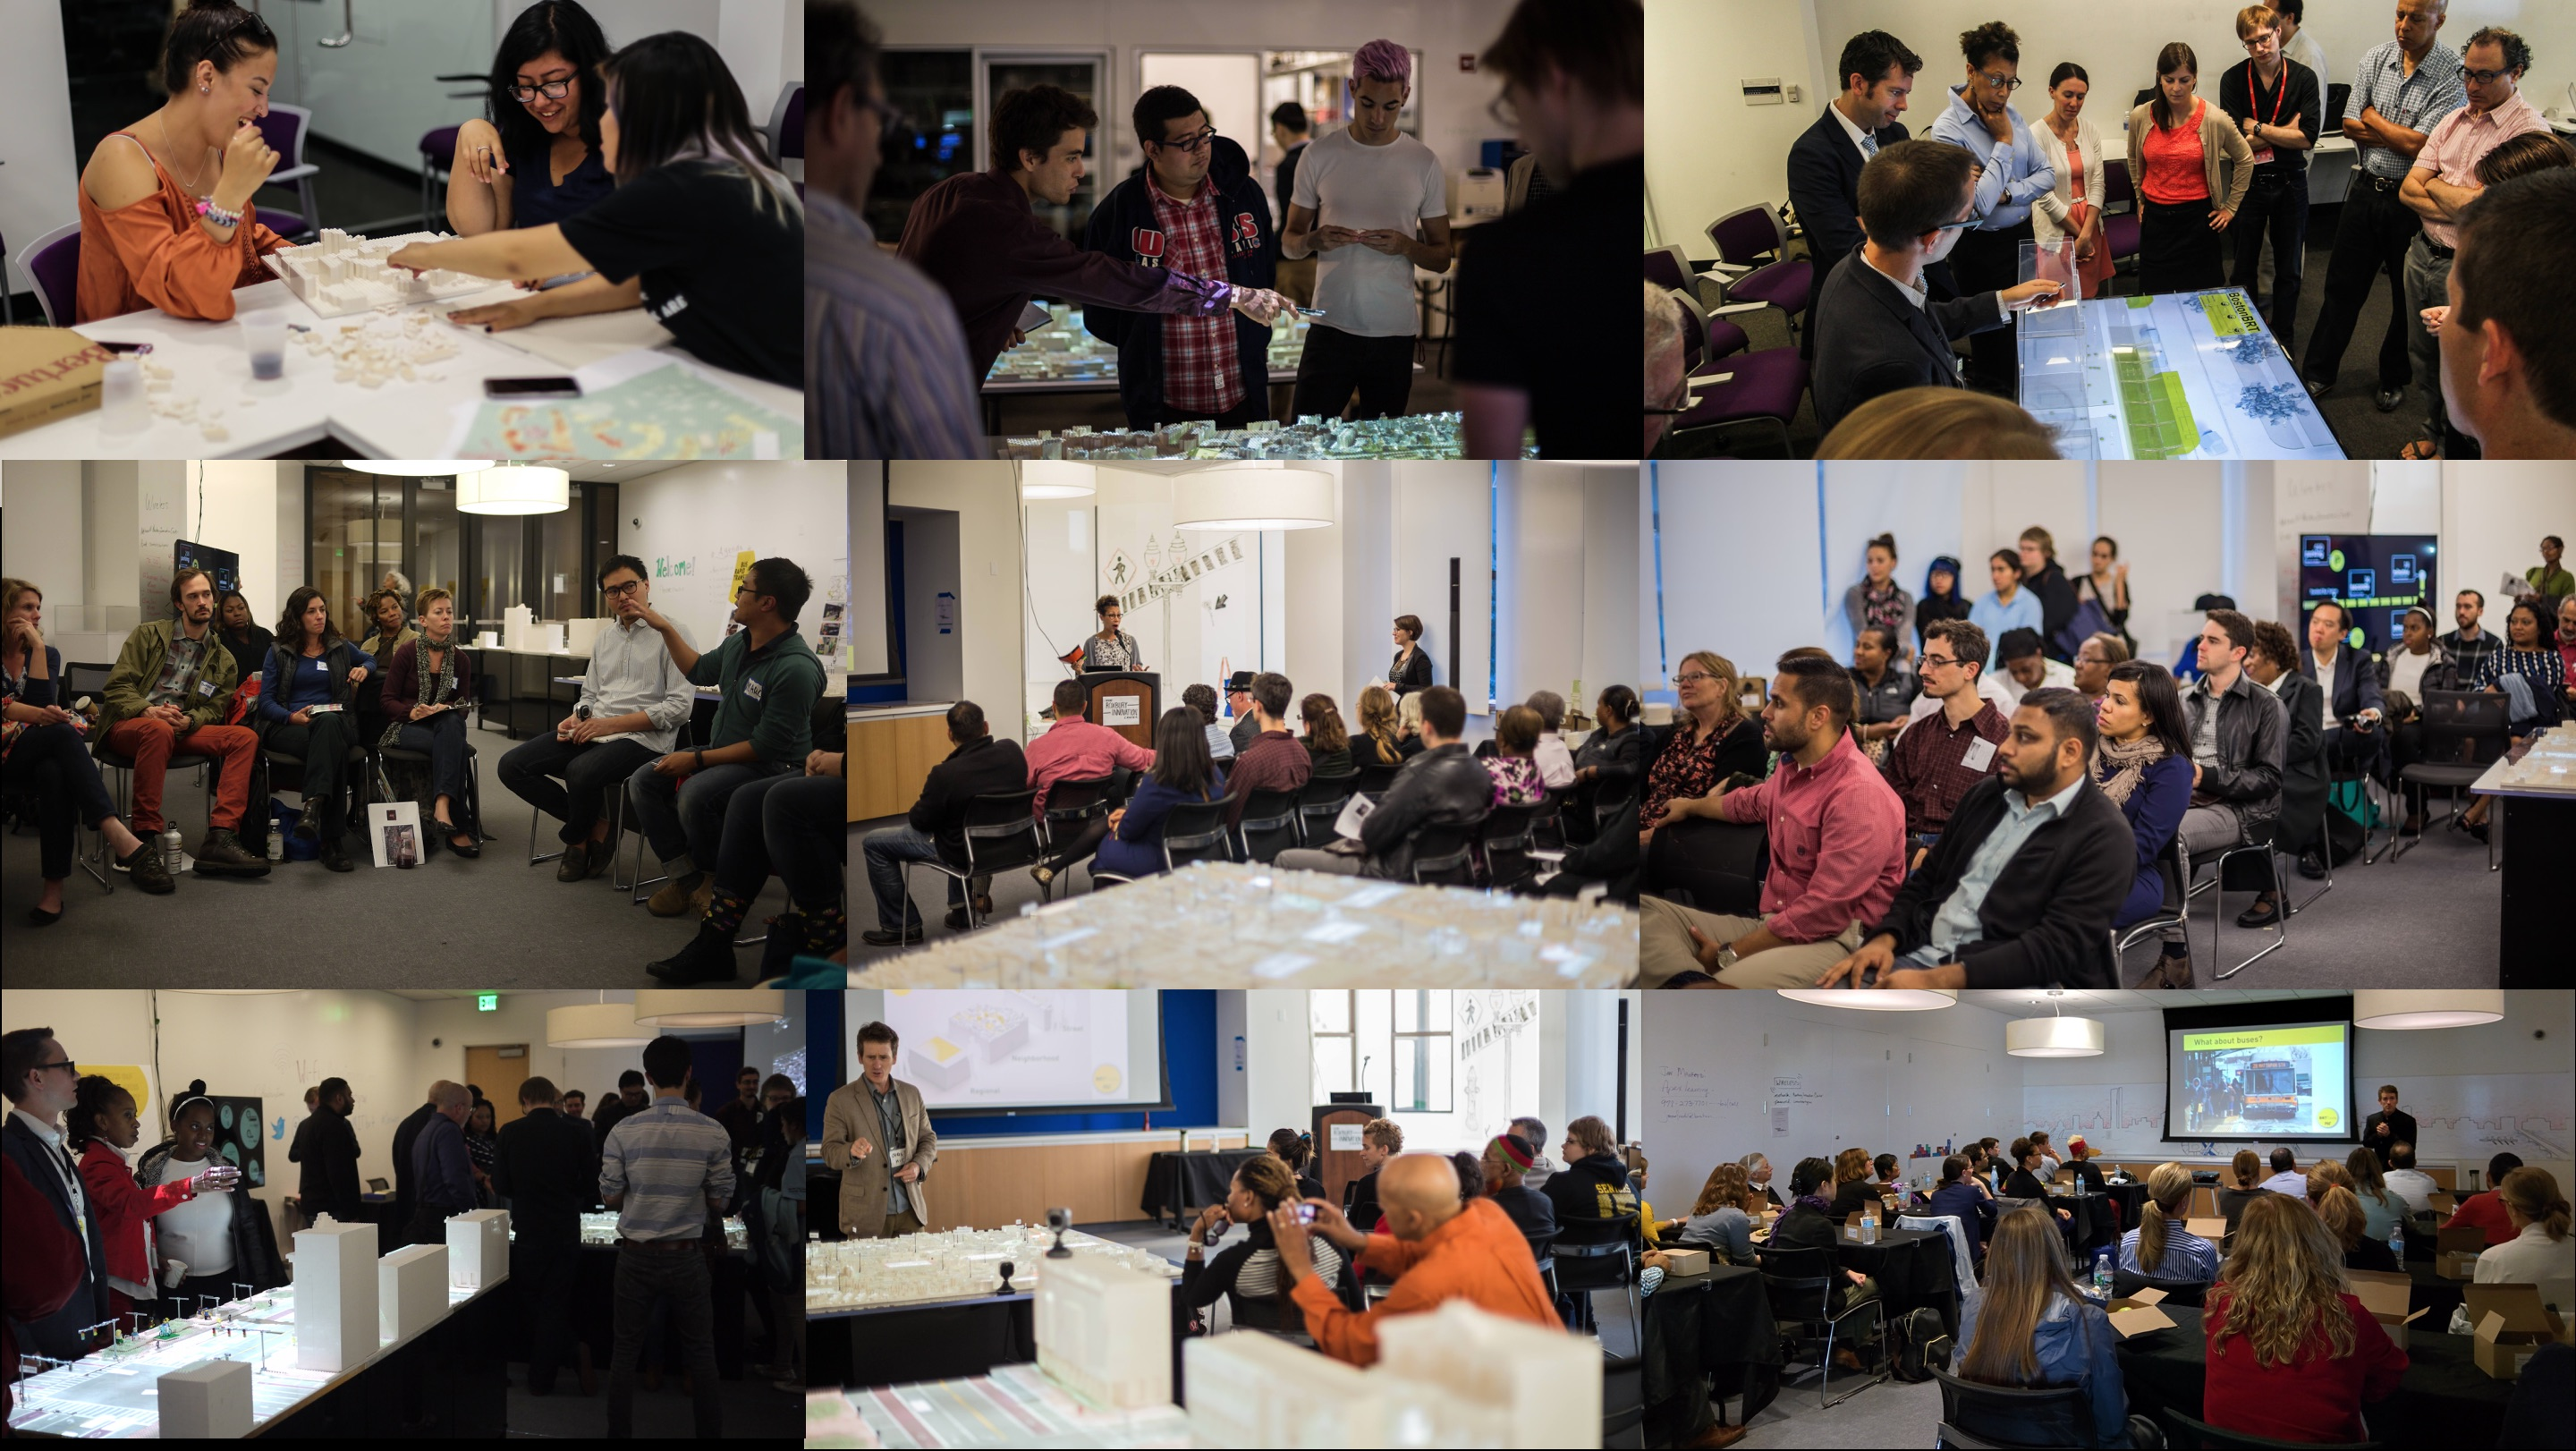
\includegraphics[width=1\textwidth]{chapters/consensus/BRT/figures/brt8.jpeg}
            \end{center}
            \caption{The many faces of public participation. A key aspect of this project was the engagement of stakeholders and the general public in every phase, from initiation and design to execution and evaluation.}
            \label{fig:brt_public_grid}
        \end{figure}

        \subsubsection{Workshops Agenda}
        {
            All six workshops followed a similar structure:
            \newline
            \textbf{Registration:} As participants entered, they were asked to register, which included reading and signing a consent to participate in the research and filling out a pre-workshop survey. Participants were also asked to use a tablet to map their points of interest (e.g., home, work, school, recreation, and healthcare locations) saved for later use in the workshop with the CoAXs tool. Participants were then asked to freely wander and familiarize themselves with the facilitators, space, and tools.
            \newline
            \textbf{Orientation:} Participants were first given an opportunity to introduce themselves to each other. One of the researchers then presented an overview to transportation issues facing Boston and the Roxbury neighborhood, explanation of the purpose of the project and project team, and introduction to key elements of Bus Rapid Transit systems.
            \newline
            \textbf{Exploration using BRT Tools:} Participants were divided into three groups. Each group was told to start at a particular station and then rotate to another station after 20 minutes. A member of the research team and a community facilitator from Nuestra was at each station helping to facilitate the conversation.
            \newline
            \textbf{Debrief discussion:} At the end of each workshop, all participants gathered for a facilitated debrief of the experience. One of the researchers facilitated each of these sessions with open-ended questions. Attempts were made to engage each of the participants during this closing session.
            \newline
            \textbf{Post-workshop survey:} Before leaving, participants were asked to fill out a post-workshop survey, including open-ended feedback as well as five-point Likert-type scales to report various takeouts and concerns. The survey was designed to be anonymous and was used to generate the report of the workshop.
        }

        \subsubsection{Data collection}
        {
            There were three primary methods to collect data during the workshops: (i) the written pre- and post-workshop surveys, (ii) verbal feedback provided during the debrief session, and (iii) observations and video/audio recordings. The pre-workshop survey collected some basic demographics, and a senses of previous familiarity with visual representation of information, public meetings, and Bus Rapid Transit. The post-workshop survey consisted of two sections: one asked questions about the overall experience of the workshop, and the second asked a series of identical questions about each of the three stations.
        }
    }

    \subsection{Results}
    {
        A mixed-method analysis suggests that the constructs of plausibility (credibility and fostering imagination) and alignment (discussion and teamwork) are correlated with specific interactions \cite{Alrashed2015}. These findings, while not robustly generalizable, suggest that stakeholder engagement built around collaborative tools, has the potential to improve processes of decision making in the context of city-planning. This section discusses the results of the workshops, including the analysis of the data collected from surveys and observations.


        \begin{figure}[!htb]
            \begin{center}
                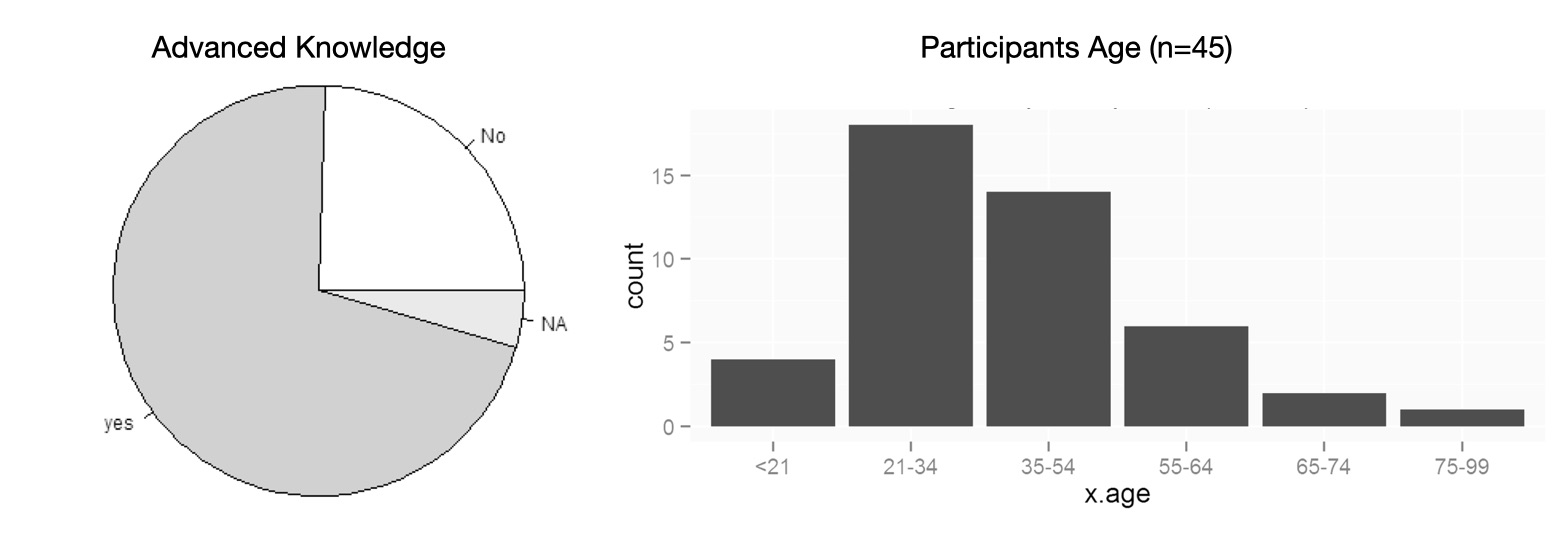
\includegraphics[width=1\textwidth]{chapters/consensus/BRT/figures/brt9.jpeg}
            \end{center}
            \caption{Participants demographic breakdown.}
            \label{fig:brt_demographics}
        \end{figure}

        \subsubsection{Participant Characteristics}
        {
            Six workshops were held with 53 total participants from a range of advocacy, policy, neighborhood, and professional organizations. Of these participants, 13 were classified as transportation, policy, or planning experts, and 15 reported attending no public planning meetings within the preceding year. Pre-workshop surveys collected basic demographics: Participants ranged in age from under 21 to over 75, though the bulk of participants were between 21 and 54. There was a diverse range of professions reported overall: About 20\% identifying as an engineer, architect, planner, transportation professional, or consultant, and 10\% identifying as a student. Almost three quarters answered yes to the question, \textit{``Are you familiar with the concept of Bus Rapid Transit (BRT)?''}
        }

        \subsubsection{Overall Responses}
        {
            Overall responses about the workshops were positive. The two questions that generated the most neutral or negative responses had to do with the role of the individual: \textit{``I helped others learn''} and \textit{``I feel that I can play an active role in the community where I live.''}
            The usage of tools was meant to assess multiple types of learning. ``Single-loop'' learning takes place when the focus is on improved techniques of efficiency (technical rationality), and goals, values, and strategies are taken for granted \cite{greenwood1998role}. The following question is taken to measure factual learning, also called `reported learning', and is associated with instrumental and strategic rationality. Nearly three quarters of participants reported positively to this question: \textit{``I learned a great deal in the workshop.''}
            \newline
            ``Double-loop'' learning is associated with communicative and value rationality. Four survey questions were used together to assess this type of learning, associated with a set of ``governing variables'': valid information, free and informed choice, internal commitment to choice, and evidence seeking behavior\footnote{Learning questions were asked for the overall workshop, since it might have been difficult for participants to isolate what they learned using an specific tool versus the workshop introduction, etc.}. The following responses signal a measure of communicative learning:

            \begin{itemize}
                \item \textit{I was able to get answers to the questions I asked} [Evidence seeking]
                \item \textit{Workshop participants discussed issues in an open way} [Valid information]
                \item \textit{Participants were open to differences in opinion} [Free and informed choice]
                \item \textit{I would support recommendations created by the participants of the workshop} [Internal commitment to choice]
            \end{itemize}

            Where valid responses were present from all questions, these were summed to create a double loop index, with possible values ranging between 4 to 20. Taken together, the answers to these questions suggest a positive response to higher-level learning. The traditional measure of the internal consistency of a scale used widely in social research, is the Cronbach alpha coefficient, which is a direct function of the number of items and their inter-correlation. The coefficient takes values between 0 and 1, and higher values correspond with higher internal consistency. An accepted rule of thumb for internal consistency, is a value of at least 0.70. The alpha value for the four statements listed above was 0.78 \cite{brown2002cronbach}.
        }

        \begin{figure}[!htb]
            \begin{center}
                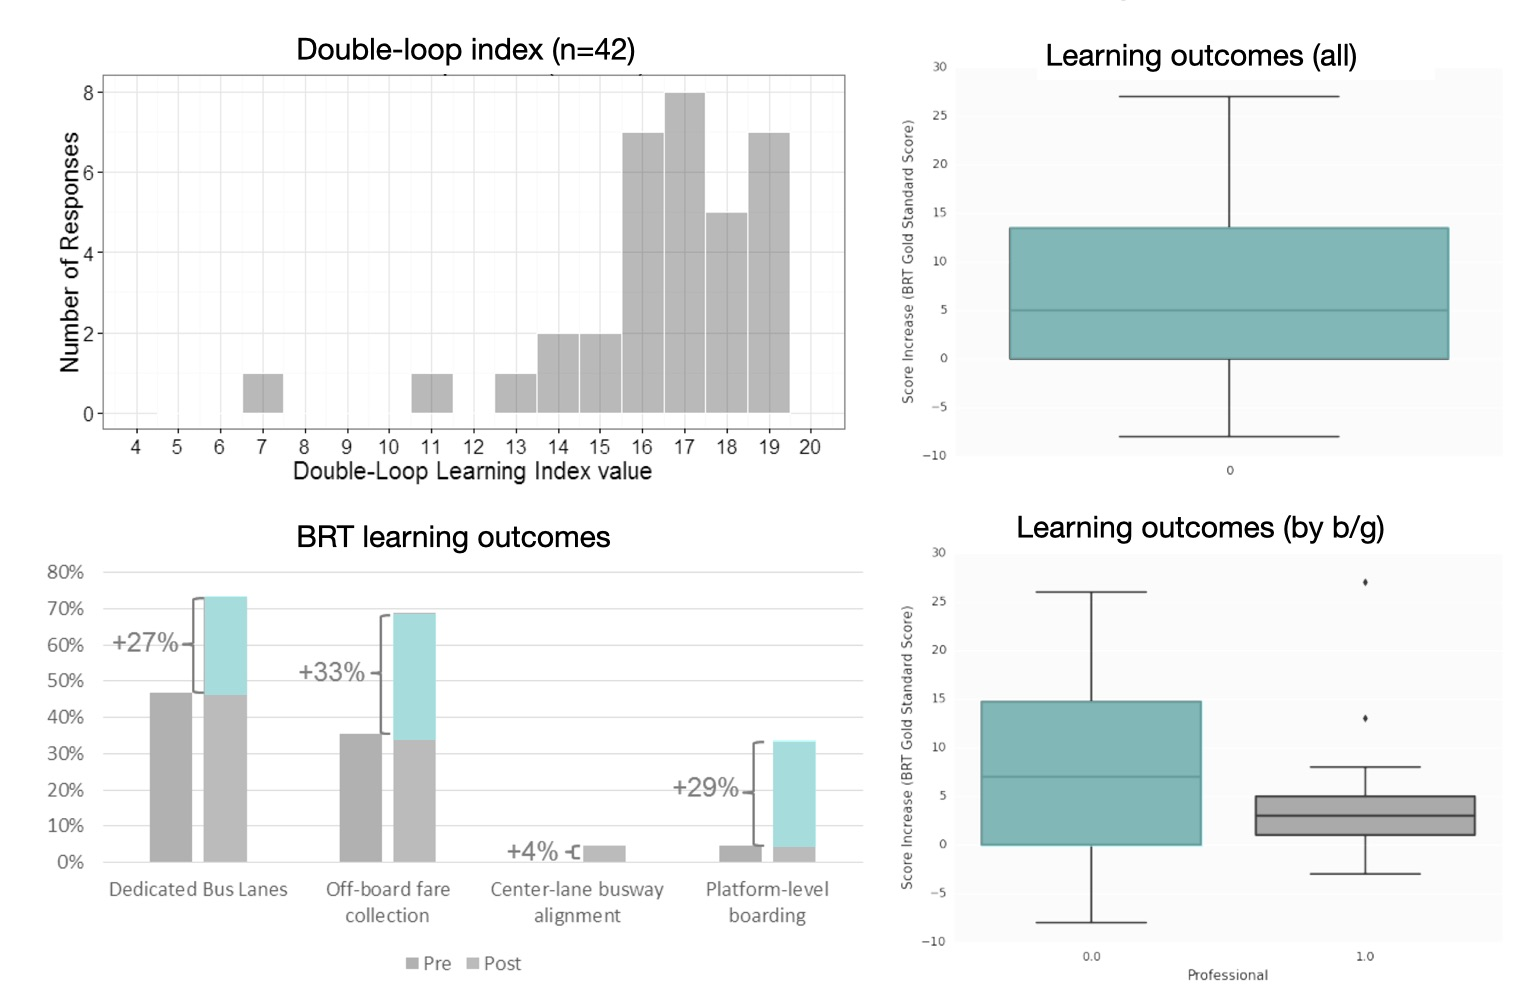
\includegraphics[width=1\textwidth]{chapters/consensus/BRT/figures/brt10.jpeg}
            \end{center}
            \caption{Learning outcomes. Overall, the vast majority of participants reported increase in `double loop' learning, awareness, and understanding of the BRT system.}
            \label{fig:brt_learning_outcomes}
        \end{figure}

        \subsubsection{Learning and Predispositions}

        {
            Participants bring with them different predispositions, such as current knowledge and attitudes. A hypothesis for this project is that the CityScope tools will encourage a different amount of learning across these differences. Responses to reported learning were segmented by past planning experiences, including along (i) expert/non-expert and (ii) skeptic/non-skeptic lines. Neither of these distinctions was asked explicitly on the entry survey; Transportation, policy, and planning experts were identified based on participants' open-ended description of their professions. Thirteen participants (about one third) were classified as ``experts'', interpreted as coming with existing transportation planning or engineering professional experience; 32 as ``non-experts,'' interpreted as coming from another discipline or life experience.
            \newline
            In general, non-experts reported more single-loop learning. For skepticism, participants were asked how many planning meetings they had attended in the preceding year, and the number of these meetings at which they learned something about this project. The difference between the former and the latter was deemed an imputed measure of skepticism about learning in planning meetings, and participants with a difference greater than zero were classified as skeptics (a binary variable). Nearly 20\% were classified as ``skeptics''; Consistent to expectations, non-skeptics reported more single-loop learning, and few reported a ``1'' (did not learn anything in the workshop).
        }


        \begin{figure}[!htb]
            \begin{center}
                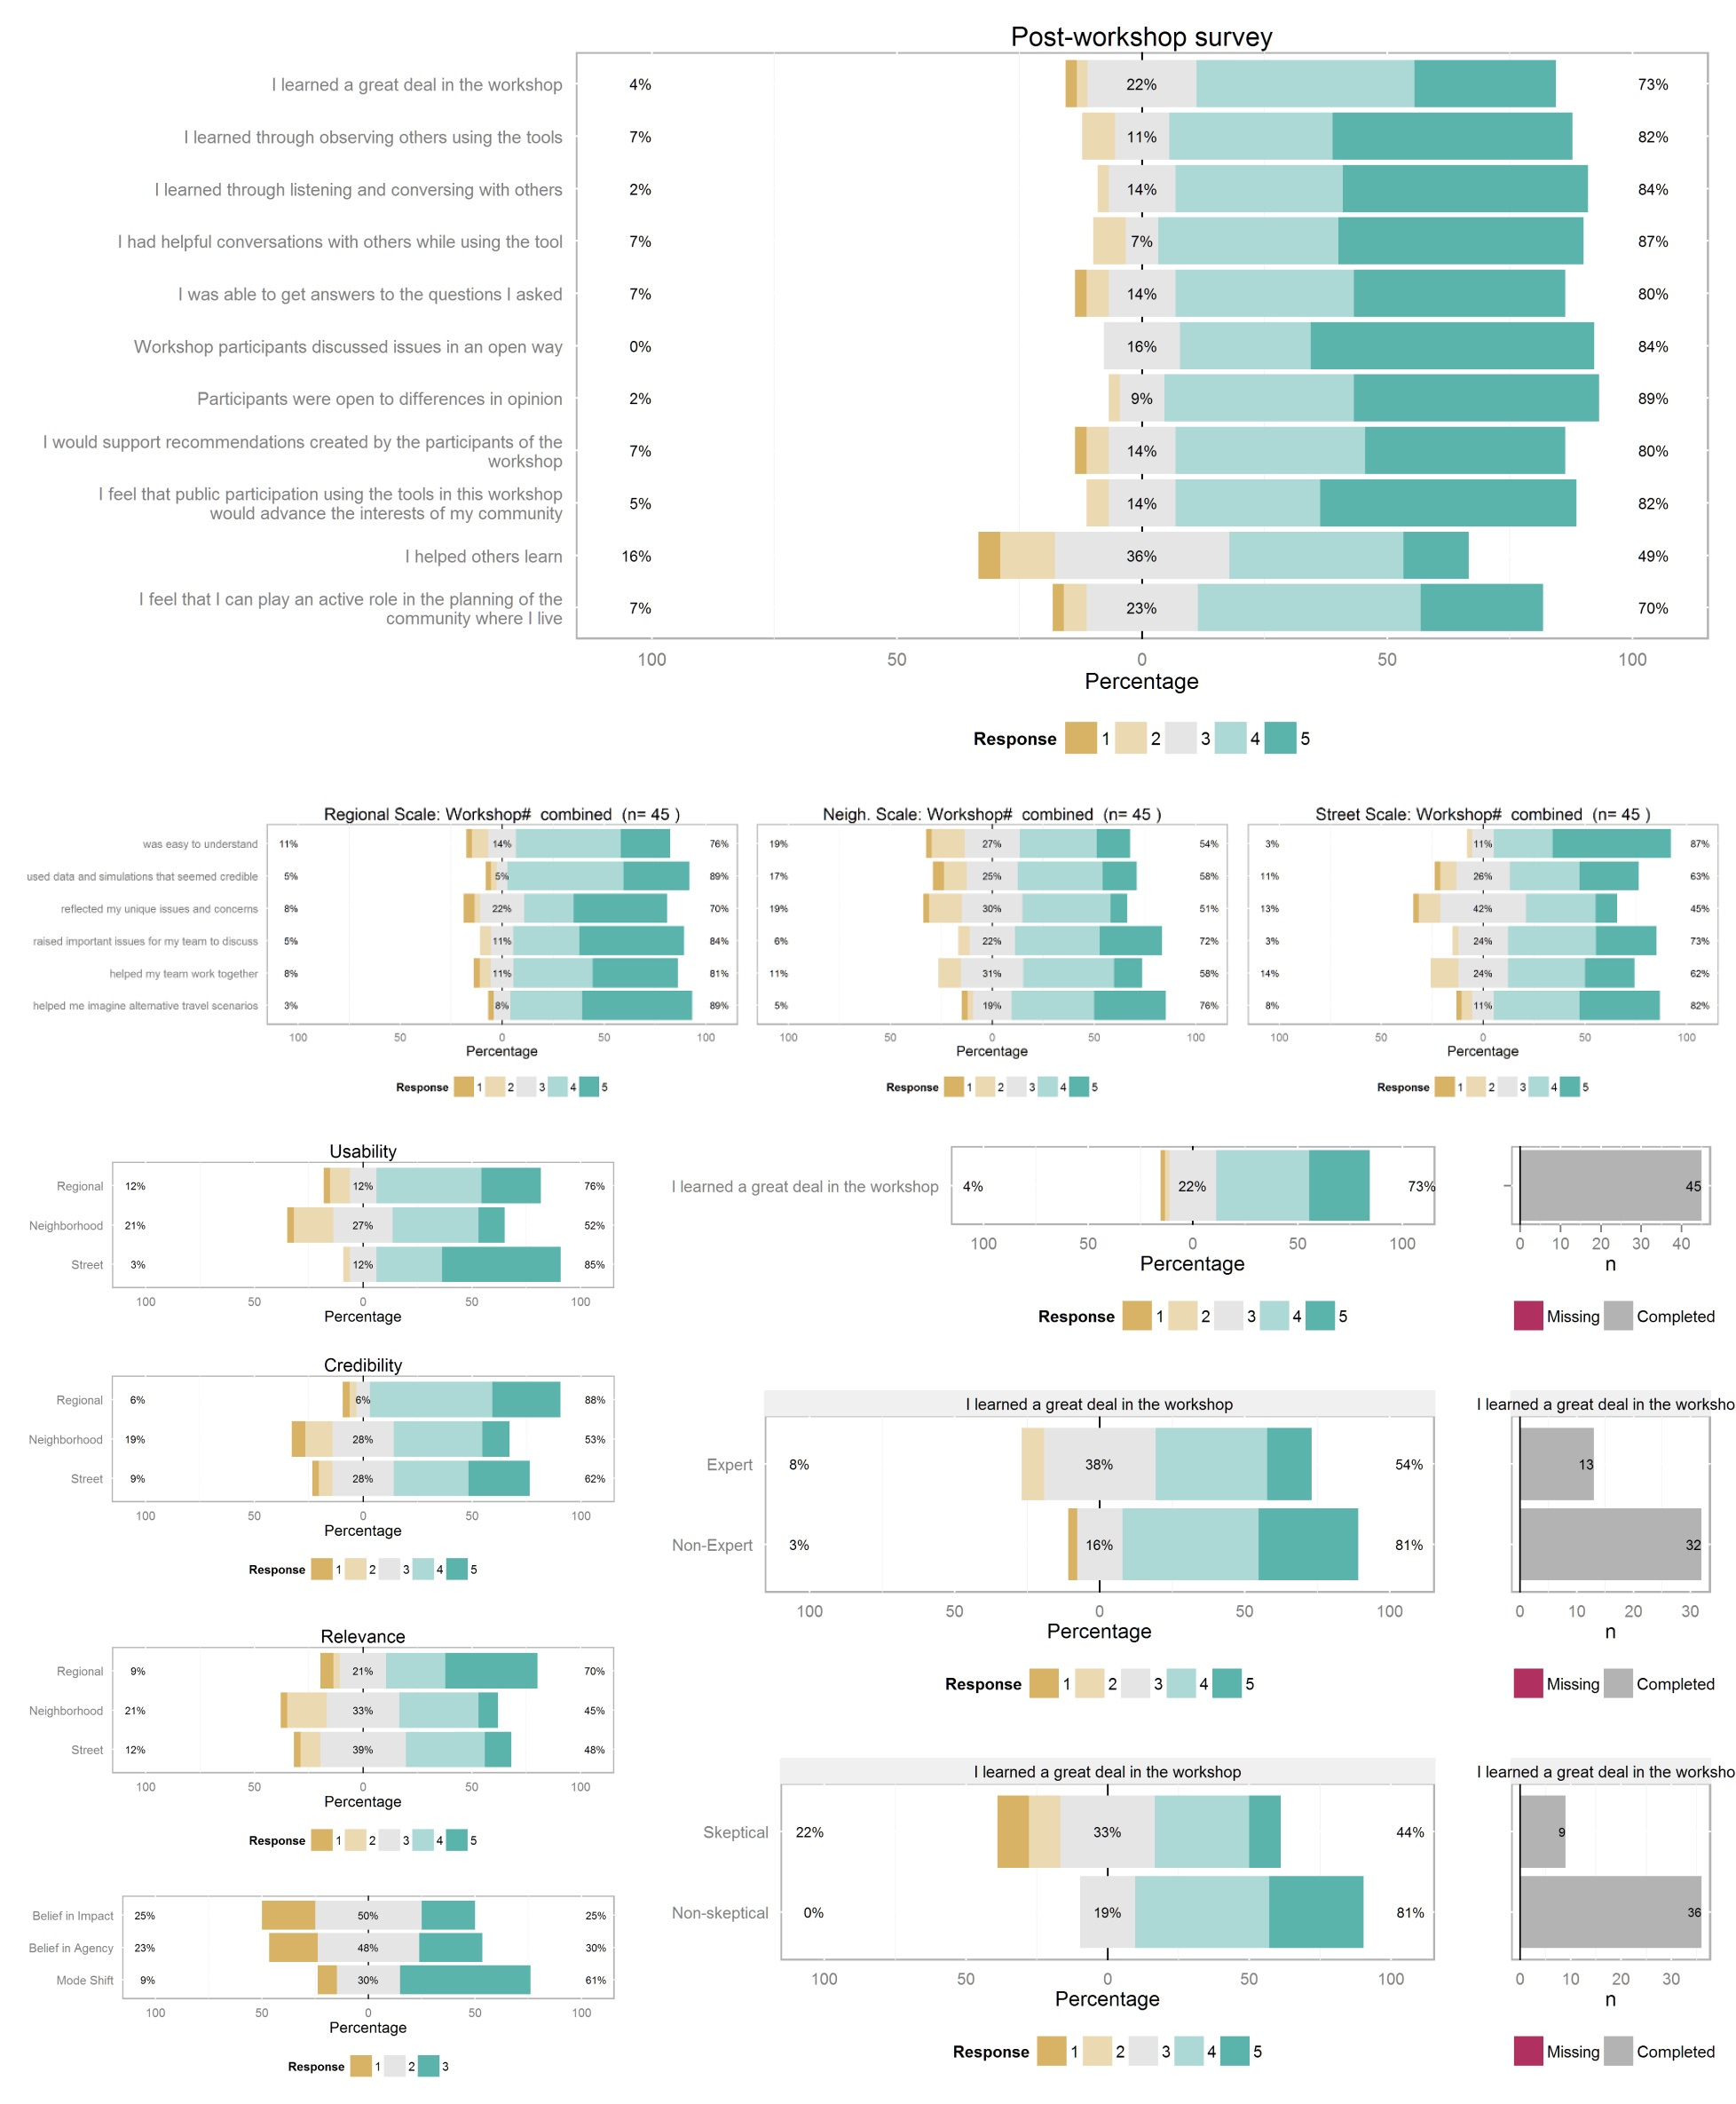
\includegraphics[width=1\textwidth]{chapters/consensus/BRT/figures/brt1.jpeg}
            \end{center}
            \caption{Aggregated results from exit surveys. Participants reflected on their learning outcomes and attitudes towards the BRT system in comparison to their initial perception. They rate each of the CityScope tools as well as cumulatively evaluate their learning from the overall experience.}
            \label{fig:brt_exit_survey}
        \end{figure}


        \subsubsection{Comparative Evaluation of Tools}
        {
            The post-workshop survey included a series of questions about each of the tools (regional, neighborhood, and street scale). Overall, the participants reported a positive experience with all tools. These are some anecdotal findings from the surveys:

            \begin{itemize}
                \item The street-scale appeared to be the easiest and most accessible to understand;
                \item The regional-scale scored the highest overall;
                \item Respondents were more ambivalent (i.e., more answering 3 on the 1-5 scale) regarding the two TUI tools.
            \end{itemize}

            The overall trends seem to hold for each of the workshops with a few exceptions. Workshop \#1 had overall higher positive feedback for the street-scale, while all the other workshops reported higher ratings for the regional scale. Workshop \#3, though, had fairly consistent ratings for each of the scales. A final observation is that Workshop \#2 held a far greater amount of negative responses overall. These point to expected peculiarities of group dynamics that are challenging to characterize after the fact.
            \newline
            Usability, relevance, and credibility are three performance metrics that were used to compare the performance of the three tools. The following three questions were used:

            \begin{itemize}
                \item Usability: \textit{``The tool was easy to understand.''}
                \item Relevance: \textit{``The tool reflected my unique issues and concerns."}
                \item Credibility: \textit{``The tool used data \& simulations that seemed credible."}
            \end{itemize}

            Participants reported the street scale to be more usable (over 50\% of responses gave the highest rating). The street scale model was intentionally designed to represent the BRT at its most literal and human-scale form. This was driven by the assumption that deep understanding of BRT systems, their impact on streetscape, and their usage pattern, are not common among the general public. It was assumed that the physical features of a BRT system poised in a familiar street, might trigger insightful feedback from the public. Key features of BRT such as prepayment gates, elevated platform, shelter and dedicated lane were clearly understandable from the model.
            \newline
            Participants reported the regional scale model to be most relevant, with almost 50\% of responses being the highest score of 5. This finding could be attributed to the fact that the regional scale tool has three unique features that enabled the participants to personalize their input and output: The participants could place icons on the map to indicate their homes and frequented destination as a form of a bookmark; choose to edit the service of a corridor of their interest; and visualize the accessibility based on a point of their interest. Participants' response for credibility at the regional scale consisted of almost 90\% of 4-5 points, with the other two scales obtaining lower scores.
        }

        \subsubsection{Assessment of Learning Outcomes}
        {
            To gain a quantitative understanding of the learning outcomes, participants were asked to identify several elements of BRT at both the entry and exit surveys (see Figure \ref{fig:brt_exit_survey} for aggregated exit survey results). Those were then matched against ITDP's BRT Standard Scorecard guidelines \cite{TheScore30:online} and assigned scores to each participant's entry and exit response for comparison\footnote{The BRT Standard is an evaluation tool for world-class bus rapid transit (BRT) based on international best practices. Despite increasing prevalence of BRT system worldwide, the characteristics of the best BRT corridors and their ability to provide levels of service more typically associated with metro and subway systems are less known. This lack of awareness frequently results in a preference for rail when BRT can be more cost-effective solution. These impressions stem partly from the lack of a common definition for BRT; Without a definition, modest improvements to standard bus service are often inaccurately labeled as BRT \cite{TheScore30:online}.}. Four of the most important elements of BRT that were most commonly reported by workshop participants include the following: (i) Dedicated Bus Lanes, (ii) Center-lane busway alignment, (iii) Platform-level boarding, and (iv) Off-board fare collection.
            \newline
            Total scores between entry and exit surveys were compared to observe the difference as proxy indicator for learning outcome. Three of the four elements above experienced an increase of about 30\%, providing some evidence that participants indeed learned about elements of BRT through the workshop. A metric for identifying overall understanding of BRT was to calculate the total score each participant would have received by the ITDP BRT scorecard both before and after the workshop\footnote{For example, one participant's response of ``Off board fare collection, designated bus lane, median busway, signal priority'', which would be treated as 8+8+2+7 = 25.}. Results indicate that participant's scores increased by an average of 5 points per person, with about 50\% of participants ranging from an increase from 0 to 14 percent.
        }

        \subsubsection{Measuring Attitude Change}
        {
            To measure whether the workshops affected each participant's attitude towards the subject matter, three questions from both entry and exit surveys were compared concerning beliefs in Agency and Impact, and the intention to increase mode usage of public transit:

            \begin{itemize}
                \item \textbf{Agency}: \textit{``I can play an active role in the planning of the community where I live''}
                \item \textbf{Impact}: \textit{``Public participation in planning advances the interests of my community''}
                \item \textbf{Mode usage of transit}: \textit{``in the last week, how many times did you travel by: car; subway/train; bus''}. This question was compared with \textit{``if corridors like we discussed today are implemented, do you imagine yourself changing the way you travel? If so, how many times per week would you travel by: car; subway/train; bus''.}
            \end{itemize}

            When assessing negative, zero, and positive change across the three questions, an increased frequency in the usage of public transit per week among over \%50 of the responses was observed, indicating a potential change in attitude toward public transit. For the beliefs in Impact and Agency, however, nearly half of responses were neutral, and the other half split across positive change and negative change. These findings were not expected, and indicate evidence that the tools and the workshop as delivered in this pilot did not show an elevation of individual's perception of agency and impact. Participants were not certain that they could indeed play a more active role in planning, or an increased sense that public participation in planning processes results in better outcomes for their community. While disappointing, it is a useful finding and points to several takeouts for future collaborative planning sessions: (i) There's a need to clearly expose the underlying mechanisms though which the tools could be modified to improve agency and impact; (ii) A line should be clearly drawn between how these sessions and tools will eventually impact decision-making and key stakeholders; (iii) The goal of learning is not sufficient in order to cerate sense of ownership and shared power amongst participants \cite{arnstein1969ladder, innes2010planning, Innes2016}.
        }

        \begin{figure}[!htb]
            \begin{center}
                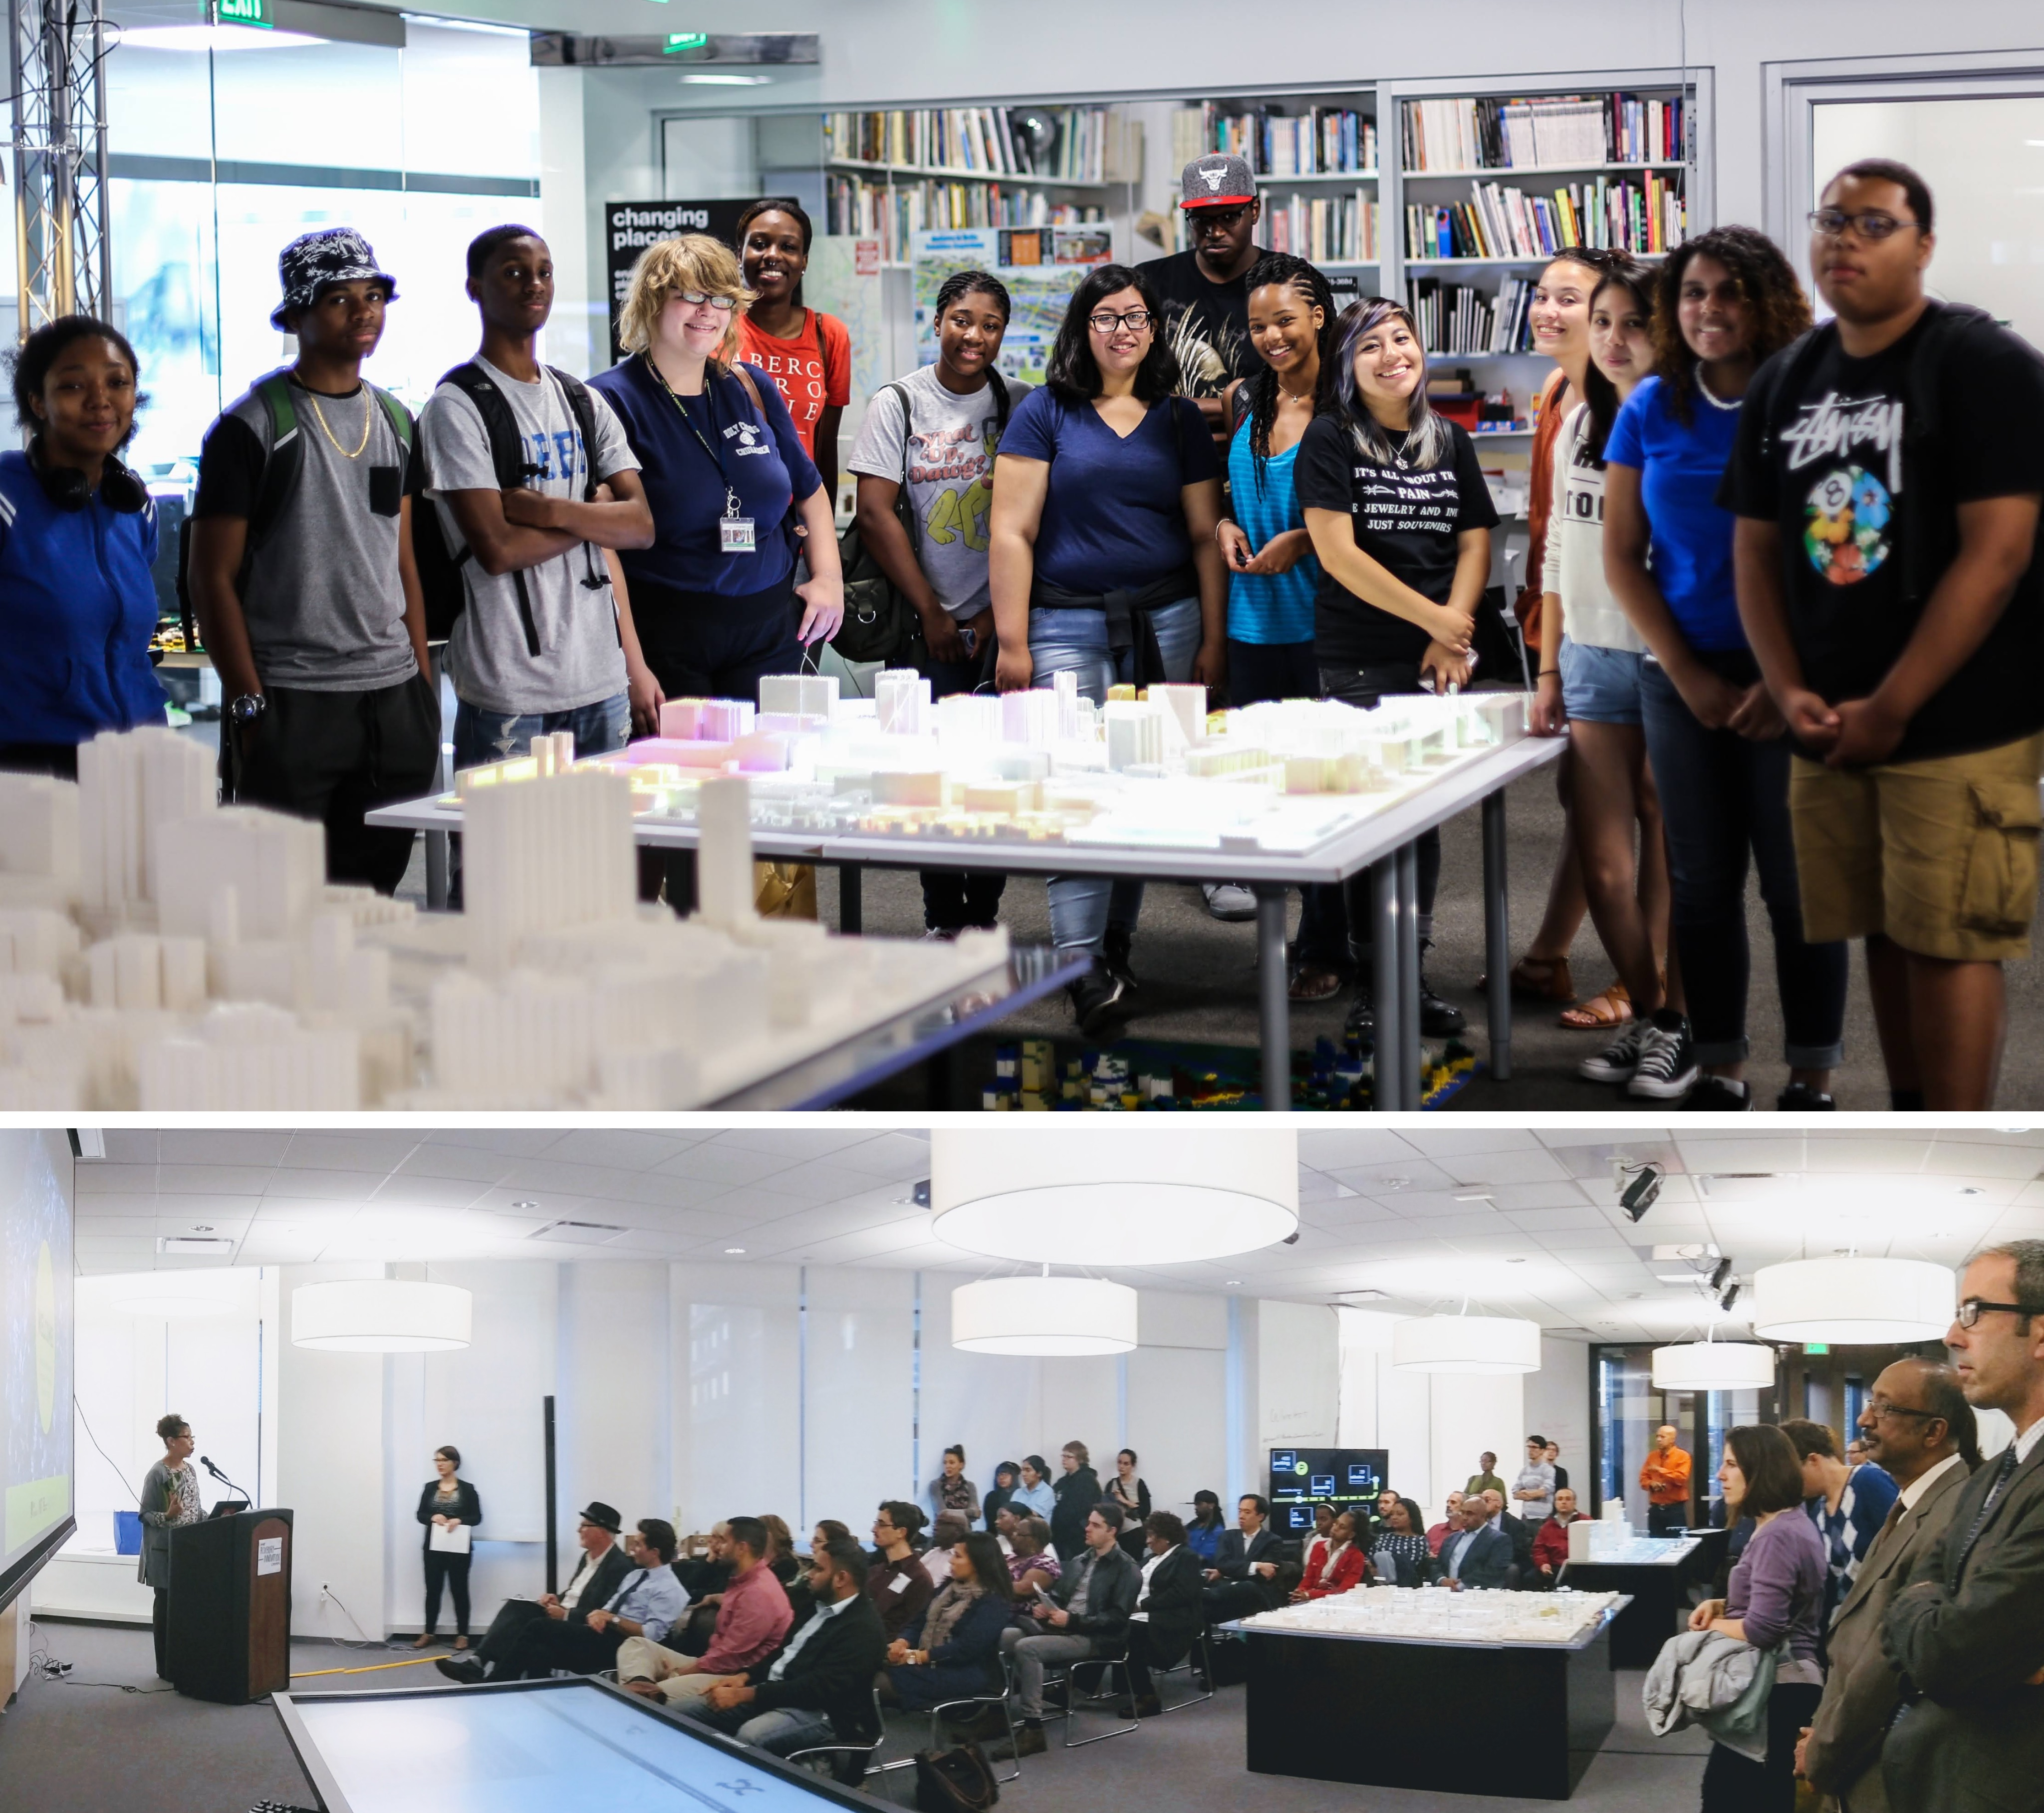
\includegraphics[width=1\textwidth]{chapters/consensus/BRT/figures/brt5.jpeg}
            \end{center}
            \caption{`Citizen Experts'. (top) MLK Scholars students constructed the TUI for two CityScope instances; Later, some of them took active roles in the guidance and operation of the tools during the workshops. (bottom) Typical BRT workshop, including the community members, the Barr Foundation, the City of Boston, and the CityScope teams.}
            \label{fig:brt_workshop}
        \end{figure}

        \subsection{Conclusion}
        {
            The BRT project was one of the first attempts to deploy CityScope tools in a real-world public participation context. The project highlighted many of the advantages as well as challenges of using novel technology in-lieu of traditional planning and participation methods. The multitude of platforms, interfaces, and methods created an opportunity to thoroughly examine the pros and cons of proposed interventions, as well as each of the tools. Specifically, the usage of an accurate, yet challenging to handle tool (such as the CoAXs), created a divide amongst users. On the other hand, tools such as the CityScope Street Scale demonstrated clarity and ease of use, but lacked variability and industry-standard rigor.
            \newline
            From a technical standpoint, the feedback showed that certain tools and interactions required different degrees of guidance and attention in order to function as designed. When it comes to community meetings, the degree of suspicion and disbelief tends to be high; Tools which can be perceive as overly sophisticated might yield opposite results than traditional tools \cite{Innes2016, ben-joseph2001}. Moreover, the BRT project highlighted a need for uniformity and cohesion amongst CityScope tools. The three platforms were initially designed to communicate and share user-inputs and analytics in real-time, but gaps and variability in their architecture hindered these efforts. The idea of a networked and standardized CityScope would grow out of this need, and will evolve into CityScopeAR \eqref{sec:cityscope_ar}, cityIO \eqref{subsec:csarch-cityio}, CityScopeJS, and the CityScope Schema \eqref{sec:cityscope_architecture}.
            \newline
            Finally, the BRT project demonstrated a real-world application for an intuitive, real-time, urban decision-support platform. It has proven that such technologies can support learning and buy-in processes, as well as help building consensus amongst different stakeholders. In the following FindingPlaces project \eqref{sec:findingplaces}, many of these notions were put to test in the challenging context of refugee housing in Germany.
        }
    }
}

